\subsection{\texorpdfstring{SYSTEMS OF TYPE \(C_{l}\) (\(l \geqslant 2\))}{SYSTEMS OF TYPE C\_l (l >= 2)}}

\begin{enumerate}
\def\labelenumi{(\Roman{enumi})}
\item
  The existence of root systems of type \(C_{l}\) has been proved in no. 5, since we have seen that the inverse system of a system of type \(B_{l}\) is of type \(C_{l}\) . A root system of type \(C_{l}\) is thus obtained by taking in \(R^{l}\) the vectors \(\pm2\varepsilon_{i}\ (1\leqslant i\leqslant l)\) , and \(\pm\varepsilon_{i}\pm\varepsilon_{j}\ (1\leqslant i<j\leqslant l)\) . The number of roots is \(2l^{2}\) .
\item
  A basis of R can be obtained by taking the image under the map \(\alpha\mapsto\frac{2\alpha}{(\alpha|\alpha)}\) of the basis of the system considered in no. 5. We obtain:
\end{enumerate}

\[
\alpha_ {1} = \varepsilon_ {1} - \varepsilon_ {2}, \alpha_ {2} = \varepsilon_ {2} - \varepsilon_ {3}, \dots , \alpha_ {l - 1} = \varepsilon_ {l - 1} - \varepsilon_ {l}, \alpha_ {l} = 2 \varepsilon_ {l}.
\]

The positive roots are the \(2\varepsilon_{i}\) and the \(\varepsilon_{i} \pm \varepsilon_{j} (i < j)\) .

\begin{enumerate}
\def\labelenumi{(\Roman{enumi})}
\setcounter{enumi}{2}
\item
  The Coxeter number is the same as for the inverse system: \(h = 2l\) .
\item
  Let \(\tilde{\alpha}=2\varepsilon_{1}=2\alpha_{1}+2\alpha_{2}+\cdots+2\alpha_{l-1}+\alpha_{l}\) , which is a root. The sum of its coordinates relative to \((\alpha_{i})\) is 2l-1=h-1. Hence, \(\tilde{\alpha}\) is the highest root. We have \((\tilde{\alpha}|\alpha_{i})=0\) for \(i\neq l\) , \((\tilde{\alpha}|\alpha_{l})=2\) . Thus, the completed Dynkin graph is
\end{enumerate}

\[
\alpha_ {1} \quad \alpha_ {2} \quad \dots \quad \alpha_ {l - 2} \quad \alpha_ {l - 1} \quad \alpha_ {l}
\]

\begin{enumerate}
\def\labelenumi{(\Alph{enumi})}
\setcounter{enumi}{21}
\tightlist
\item
  We have already determined \(R^{-}\) , which is of type \(B_{l}\) . By formula (19) of § 1, no. 12 and by no. 5 (V), the square of the length of \(2\varepsilon_{i}\) for \(\Phi_{R}\) is
\end{enumerate}

\[
((l + 1) (4 l - 2)) ^ {+ 1} ((4 l - 2) ^ {- 1}) ^ {- 1} = (l + 1) ^ {- 1};
\]

thus, \(\Phi_{\mathrm{R}}(x,y) = (x|y) / 4(l + 1)\) .

We have \(\gamma(R) = \gamma(R') = (l + 1)(4l - 2)\) .

\begin{enumerate}
\def\labelenumi{(\Roman{enumi})}
\setcounter{enumi}{5}
\tightlist
\item
  The fundamental weights are easily found:
\end{enumerate}

\[
\begin{array}{l} \omega_ {i} = \varepsilon_ {1} + \varepsilon_ {2} + \dots + \varepsilon_ {i} \\ = \alpha_ {1} + 2 \alpha_ {2} + \dots + (i - 1) \alpha_ {i - 1} + i (\alpha_ {i} + \alpha_ {i + 1} + \dots + \frac {1}{2} \alpha_ {l}) (i \leqslant l). \end{array}
\]

\begin{enumerate}
\def\labelenumi{(\Roman{enumi})}
\setcounter{enumi}{6}
\tightlist
\item
  The sum of the positive roots is
\end{enumerate}

\[
\begin{array}{r l} 2 \rho & = 2 l \varepsilon_ {1} + (2 l - 2) \varepsilon_ {2} + \dots + 4 \varepsilon_ {l - 1} + 2 \varepsilon_ {l} \\ & = 2 l \alpha_ {1} + 2 (2 l - 1) \alpha_ {3} + \dots + i (2 l - i + 1) \alpha_ {i} + \dots \\ & \qquad \dots + (l - 1) (l + 2) \alpha_ {l - 1} + \frac {1}{2} l (l + 1) \alpha_ {l}. \end{array}
\]

\begin{enumerate}
\def\labelenumi{(\Roman{enumi})}
\setcounter{enumi}{7}
\item
  By no. 4 and no. 5 (VIII), \(Q(R) = L_{1}\) , \(P(R) = L_{0}\) ; \(P(R)/Q(R)\) is isomorphic to Z/2Z, and the connection index is 2.
\item
  and (X) These data depend only on W(R), and so are the same as for type \(B_{l}\) .
\item
  The same argument as in no. 5 shows that \(A(R) = W(R)\) and \(w_0 = -1\) .
\item
  The single non-identity element of \(\mathrm{P}(\mathrm{R}^{-})/\mathrm{Q}(\mathrm{R}^{-})\) defines the unique non-trivial automorphism of the completed Dynkin graph: it interchanges the vertices corresponding to \(\alpha_{j}\) and \(\alpha_{l-j}\) for \(0 \leqslant j \leqslant l\) .
\end{enumerate}

\subsection{\texorpdfstring{SYSTEMS OF TYPE \(\mathbf{A}_l\) (\(l \geqslant 1\))}{SYSTEMS OF TYPE A\_l (l >= 1)}}

\begin{enumerate}
\def\labelenumi{(\Roman{enumi})}
\tightlist
\item
  and (II) Let \(V\) be the hyperplane in \(E = R^{l + 1}\) with equation \(\sum_{i=1}^{l + 1} \xi_i = 0\) . Replacing \(l\) by \(l + 1\) in no. 5, we obtain a system \(R'\) of type \(B_{l + 1}\) in \(E\) with basis
\end{enumerate}

\[
\alpha_ {1} = \varepsilon_ {1} - \varepsilon_ {2}, \alpha_ {2} = \varepsilon_ {2} - \varepsilon_ {3}, \dots , \alpha_ {l} = \varepsilon_ {l} - \varepsilon_ {l + 1}. \alpha_ {l + 1} = \varepsilon_ {l + 1}.
\]

Since \(\alpha_{1},\ldots,\alpha_{l}\) generate V, \(R=R^{\prime}\cap V\) is a root system in V with basis \((\alpha_{1},\ldots,\alpha_{l})\) (§ 1, no. 7, Cor. 4 of Prop. 20). By the calculation of the scalar products in no. 5, it is immediate that R is of type \(A_{l}\) . The elements of R are the \(\varepsilon_{i}-\varepsilon_{j}\) ( \(i\neq j,1\leqslant i\leqslant l+1,1\leqslant j\leqslant l+1\) ). There are \(n=l(l+1)\) roots. The positive roots are the \(\varepsilon_{i}-\varepsilon_{j}\) where \(i<j\) .

\begin{enumerate}
\def\labelenumi{(\Roman{enumi})}
\setcounter{enumi}{2}
\item
  We have \(h = n / l = l + 1\) .
\item
  Let \(\tilde{\alpha} = \varepsilon_1 - \varepsilon_{l+1} = \alpha_1 + \alpha_2 + \cdots + \alpha_l\) , which is a root. The sum of its coordinates relative to \((\alpha_i)\) is \(l = h - 1\) . Hence \(\tilde{\alpha}\) is the highest root.
\end{enumerate}

For \(l = 1\) . \(\tilde{\alpha} = \alpha_{1}\) so \((\tilde{\alpha}|\alpha_{1}) = 2\) ; the Coxeter graph of the group \(W_{a}(R)\) is

For \(l \geqslant 2\) , \((\tilde{\alpha}|\alpha_i) = 0\) for \(0 < i < l\) and \((\tilde{\alpha}|\alpha_1) = (\tilde{\alpha}|\alpha_l) = 1\) . Hence the completed Dynkin graph is:

\pandocbounded{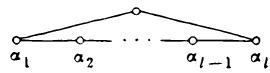
\includegraphics[keepaspectratio]{images/part002_36cfe44b.jpg}}

\begin{enumerate}
\def\labelenumi{(\Alph{enumi})}
\setcounter{enumi}{21}
\tightlist
\item
  Identifying V with its dual using the scalar product, we have \(\alpha^{\prime} = \frac{2\alpha}{(\alpha|\alpha)} = \alpha\) for all \(\alpha \in R\) , so \(R^{\prime} = R\) .
\end{enumerate}

For the form \(\Phi_{\mathbb{R}}\) , the length of the roots is \(h^{-1/2} = (l + 1)^{-1/2}\) (§ 1, no. 12); so \(\Phi_{\mathrm{R}}(x,y) = (x|y)/2(l+1)\) .

We have \(\gamma (\mathbb{R}) = (l + 1)^2\) (§ 1. no. 12, formula (20)).

\begin{enumerate}
\def\labelenumi{(\Roman{enumi})}
\setcounter{enumi}{5}
\tightlist
\item
  Let \((\omega_{i})_{1\leqslant i\leqslant l}\) be the family of fundamental weights. Put
\end{enumerate}

\[
\omega_ {i} = \sum_ {j = 1} ^ {l + 1} \xi_ {i j} \varepsilon_ {j}. \quad \text { with } \xi_ {i j} \in \mathbf {R}.
\]

The conditions \((\omega_{i}|\alpha_{j}) = \delta_{ij}\) and \(\omega_{i}\in V\) give

\[
\xi_ {i i} - \xi_ {i, i + 1} = 1, \quad \xi_ {i j} - \xi_ {i, j + 1} = 0 \text {   for   } j \neq i, \quad \sum_ {j = 1} ^ {l + 1} \xi_ {i j} = 0,
\]

which easily lead to

\[
\begin{array}{r l} \omega_ {i} & = \varepsilon_ {1} + \dots + \varepsilon_ {i} - \frac {i}{l + 1} (\varepsilon_ {1} + \dots + \varepsilon_ {l + 1}) \\ & = \frac {1}{l + 1} ((l - i + 1) (\alpha_ {1} + 2 \alpha_ {2} + \dots + (i - 1) \alpha_ {i - 1}) \\ & \quad + i ((l - i + 1) \alpha_ {i} + (l - i) \alpha_ {i + 1} + \dots + \alpha_ {l})). \end{array}
\]

\begin{enumerate}
\def\labelenumi{(\Roman{enumi})}
\setcounter{enumi}{6}
\tightlist
\item
  The sum of the positive roots is
\end{enumerate}

\[
\begin{array}{r l} 2 \rho & = l \varepsilon_ {1} + (l - 2) \varepsilon_ {2} + (l - 4) \varepsilon_ {3} + \dots - (l - 2) \varepsilon_ {l} - l \varepsilon_ {l + 1} \\ & = l \alpha_ {1} + 2 (l - 1) \alpha_ {2} + \dots + i (l - i + 1) \alpha_ {i} + \dots + l \alpha_ {l}. \end{array}
\]

\begin{enumerate}
\def\labelenumi{(\Roman{enumi})}
\setcounter{enumi}{7}
\tightlist
\item
  Introduce in \(\mathbf{E} = \mathbf{R}^{l + 1}\) the subgroup \(\mathrm{L}_0\) of no. 4. Let \(p\) be the orthogonal projection of E onto V. By § 1, no. 10, Prop. 28, we have
\end{enumerate}

\[
\mathrm{Q} (\mathrm{R}) = \mathrm{Q} \left(\mathrm{R} ^ {\prime}\right) \cap \mathrm{V} \neq \mathrm{L} _ {0} \cap \mathrm{V}, \text { and } \mathrm{P} (\mathrm{R}) = p \left(\mathrm{P} \left(\mathrm{R} ^ {\prime}\right)\right);
\]

in view of the fact that the last fundamental weight of \(R'\) is orthogonal to V, we have \(\mathrm{P}(\mathrm{R}) = p(\mathrm{Q}(\mathrm{R}')) = p(\mathrm{L}_0)\) . Thus, \(\mathrm{P}(\mathrm{R})\) is the group generated by the \(\varepsilon_i - \varepsilon_j\) and by \(p(\varepsilon_1) = \varepsilon_1 \to (l + 1)^{-1} \sum_{i=1}^{l+1} \varepsilon_i\) , so

\[
\mathrm{P} (\mathrm{R}) = \mathrm{Q} (\mathrm{R}) + \mathbf {Z} \left(\varepsilon_ {1} - (l + 1) ^ {- 1} \sum_ {i = 1} ^ {l + 1} \varepsilon_ {i}\right).
\]

Now \(l + 1\) is the smallest integer \(m > 0\) such that \(mp(\varepsilon_1) \in Q(R)\) . Thus \(P(R)/Q(R)\) is isomorphic to \(\mathbf{Z}/(l + 1)\mathbf{Z}\) and the connection index is \(l + 1\) .

\begin{enumerate}
\def\labelenumi{(\Roman{enumi})}
\setcounter{enumi}{8}
\tightlist
\item
  and (X) For any automorphism g of V, let \(\varphi(g)\) be the automorphism of E that extends g and leaves \(\varepsilon_{1} + \varepsilon_{2} + \cdots + \varepsilon_{l}\) invariant. If g is the orthogonal reflection \(s_{\varepsilon_{i} - \varepsilon_{j}}|V\) , \(\varphi(g)\) is equal to \(s_{\varepsilon_{i} - \varepsilon_{j}}\) , which interchanges \(\varepsilon_{i}\) and \(\varepsilon_{j}\) and leaves fixed the \(\varepsilon_{k}\) with k distinct from i and j. Let
\end{enumerate}

\[
X = \left\{\varepsilon_ {1}, \varepsilon_ {2}, \dots , \varepsilon_ {l + 1} \right\}.
\]

Then \(g \mapsto \varphi(g)|_{\mathbf{X}}\) is an isomorphism from \(W(\mathbf{R})\) to the symmetric group of \(\mathbf{X}\) . Thus, \(W(\mathbf{R})\) is isomorphic to the symmetric group \(\mathfrak{S}_{l+1}\) , and so is of order \((l+1)!\) .

The symmetric algebra \(\mathbf{S}(\mathrm{E})\) can be identified canonically with the algebra of polynomial functions \(\mathrm{P}(\xi_1, \xi_2, \ldots, \xi_{l+1})\) on E. Let \(\mathrm{G} = \varphi(\mathrm{W}(\mathrm{R}))\) . By the preceding paragraph, the set \(\mathbf{S}(\mathrm{E})^{\mathrm{G}}\) of elements of \(\mathbf{S}(\mathrm{E})\) invariant under G is the set of symmetric polynomials (Algebra, Chap. V, App. I), and consequently (ibid.) is the algebra generated by the functions

\[
s _ {i} ^ {\prime} = \sum_ {\tau \in \mathfrak {S} _ {l + 1}} \xi_ {\tau (1)} \xi_ {\tau (2)} \dots \xi_ {\tau (i)} \quad (1 \leqslant i \leqslant l + 1).
\]

The algebra \(\mathbf{S}(\mathrm{V})\) can be identified with the restrictions to \(\mathrm{V}\) of the polynomial functions on \(\mathrm{E}\) . If \(\mathrm{P} \in \mathbf{S}(\mathrm{E})^{\mathrm{G}}\) , the restriction of \(\mathrm{P}\) to \(\mathrm{V}\) is clearly invariant under \(\mathrm{W}(\mathrm{R})\) . Conversely, if \(\mathrm{Q} \in \mathbf{S}(\mathrm{V})^{\mathrm{W}(\mathrm{R})}\) , there exists \(\mathrm{P} \in \mathbf{S}(\mathrm{E})\) extending \(\mathrm{Q}\) ; replacing \(\mathrm{P}\) by \(((l + 1)!)^{-1} \sum_{g \in \mathrm{G}} g(\mathrm{P})\) , which has the same restriction as \(\mathrm{P}\) to \(\mathrm{V}\) . we can assume that \(\mathrm{P} \in \mathbf{S}(\mathrm{E})^{\mathrm{G}}\) . Thus, \(\mathbf{S}(\mathrm{V})^{\mathrm{W}(\mathrm{R})}\) is generated by the \(s_i = s_i'|\mathrm{V}\) . Now \(s_1 = 0\) . Moreover, the transcendence degree over \(\mathbf{R}\) of the field of fractions of \(\mathbf{S}(\mathrm{V})^{\mathrm{W}(\mathrm{R})}\) is \(l\) , so the \(s_i\) ( \(2 \leqslant i \leqslant l + 1\) ) are algebraically independent. Since the \(s_i\) are of degrees \(2, 3, \ldots, l + 1\) , the exponents of \(\mathrm{W}(\mathrm{R})\) are

\[
1, 2, 3, \dots , l.
\]

\begin{enumerate}
\def\labelenumi{(\Roman{enumi})}
\setcounter{enumi}{10}
\tightlist
\item
  For \(l = 1\) . A(R) = W(R) = Z/2Z and \(w_0 = -1\) .
\end{enumerate}

For \(l \geqslant 2\) , let \(\varepsilon \in A(R)\) be the automorphism that transforms \(\alpha_i\) to \(\alpha_{l+1-i}\) . It is clear that the automorphism induced by \(\varepsilon\) is the unique non-trivial automorphism of the Dynkin graph. The group \(A(R)/W(R)\) is isomorphic to \(Z/2Z\) . Since -1 is an element of \(A(R)\) which does not belong to \(W(R)\) by (IX) and (X), we see that \(A(R)\) is isomorphic to \(W(R) \times Z/2Z\) . We have \(w_0 = -\varepsilon\) .

\begin{enumerate}
\def\labelenumi{(\Roman{enumi})}
\setcounter{enumi}{11}
\tightlist
\item
  The group \(\mathrm{P}(\mathrm{R}^{-})/\mathrm{Q}(\mathrm{R}^{-})\) is cyclic of order \(l+1\) and acts on the completed Dynkin graph by circular permutations. If \(l\geqslant2\) , the unique non-identity element of \(\mathrm{A}(\mathrm{R})/\mathrm{W}(\mathrm{R})\) acts on \(\mathrm{P}(\mathrm{R}^{-})/\mathrm{Q}(\mathrm{R}^{-})\) by the automorphism \(x\mapsto-x\) .
\end{enumerate}

\subsection{\texorpdfstring{SYSTEMS OF TYPE \(D_{l}\) (\(l \geqslant 3\))}{SYSTEMS OF TYPE D\_l (l >= 3)}}

\begin{enumerate}
\def\labelenumi{(\Roman{enumi})}
\item
  Consider in \(V = R^{l}\) the group \(L_{0}\) (no. 4). The set R of \(\alpha \in L_{0}\) such that \((\alpha|\alpha) = 2\) consists of the vectors \(\pm\varepsilon_{i} \pm \varepsilon_{j}\) ( \(1 \leqslant i < j \leqslant l\) ). It is clear that R generates V and that \(2(\alpha|\beta)/(\alpha|\alpha) \in \mathbf{Z}\) for all \(\alpha, \beta \in R\) . Thus R is a reduced root system in V (no. 4). The number of roots is \(n = 2l(l - 1)\) .
\item
  Put
\end{enumerate}

\[
\alpha_ {1} = \varepsilon_ {1} - \varepsilon_ {2}, \alpha_ {2} = \varepsilon_ {2} - \varepsilon_ {3} \dots . \alpha_ {l - 1} = \varepsilon_ {l - 1} - \varepsilon_ {l}, \alpha_ {l} = \varepsilon_ {l - 1} + \varepsilon_ {l}.
\]

The following formulas are immediate:

\[
\begin{array}{c} \varepsilon_ {i} - \varepsilon_ {j} = \alpha_ {i} + \alpha_ {i + 1} + \dots + \alpha_ {j - 1} (i <   j) \\ \varepsilon_ {i} + \varepsilon_ {j} = \alpha_ {i} + \alpha_ {i + 1} + \dots + \alpha_ {j - 1} + 2 \alpha_ {j} + 2 \alpha_ {j + 1} + \dots \\ \qquad \qquad \qquad \qquad \qquad \qquad \dots + 2 \alpha_ {l - 2} + \alpha_ {l - 1} + \alpha_ {l} (i <   j \leqslant l - 2) \\ \varepsilon_ {i} + \varepsilon_ {l - 1} = \alpha_ {i} + \alpha_ {i + 1} + \dots + \alpha_ {l} (i <   l - 1) \\ \varepsilon_ {i} + \varepsilon_ {l} = \alpha_ {i} + \alpha_ {i + 1} + \dots + \alpha_ {l - 2} + \alpha_ {l} (i <   l - 1) \\ \varepsilon_ {l - 1} + \varepsilon_ {l} = \alpha_ {l}. \end{array}
\]

so \((\alpha_{1},\ldots,\alpha_{l})\) is a basis if R (§ 1, no. 2. Cor. 3 of Prop. 20). Further, \(\| \alpha_{i}\|^{2}=2\) for all \(i\) , \((\alpha_{i}|\alpha_{j})=0\) for \(i+1<j\) except for \(i=l-2\) , \(j=l\) in which case \((\alpha_{l-2}|\alpha_{l})=-1\) , \((\alpha_{i}|\alpha_{i+1})=-1\) for \(i\leqslant l-2\) , and finally \((\alpha_{l-1}|\alpha_{l})=-1\) ; the Dynkin graph of R is thus of type D \(_{l}\) . The positive roots are the \(\varepsilon_{i}\pm\varepsilon_{j}\) for \(i<j\) .

\begin{enumerate}
\def\labelenumi{(\Roman{enumi})}
\setcounter{enumi}{2}
\item
  We have \(h = n / l = 2(l - 1)\) .
\item
  Let \(\tilde{\alpha} = \varepsilon_{1} + \varepsilon_{2} = \alpha_{1} + 2\alpha_{2} + \cdots + 2\alpha_{l-2} + \alpha_{l-1} + \alpha_{l}\) , which is a root. The sum of its coordinates relative to \((\alpha_{i})\) is
\end{enumerate}

\[
2 l - 3 = h - 1.
\]

Hence \(\tilde{\alpha}\) is the highest root.

If \(l = 3\) , we have

\[
(\tilde {\alpha} | \alpha_ {1}) = 0, \quad (\tilde {\alpha} | \alpha_ {2}) = (\tilde {\alpha} | \alpha_ {3}) = 1.
\]

If \(l \geqslant 4\) . we have \((\tilde{\alpha}|\alpha_i) = 0\) for \(i \neq 2\) and \((\tilde{\alpha}|\alpha_2) = 1\) . Hence the completed Dynkin graph is:

\[
\alpha_ {1} \quad \alpha_ {2} \quad \alpha_ {3} \quad \dots \quad \alpha_ {i - 3} \quad \alpha_ {i - 2} \quad \alpha_ {i - 1}
\]

\begin{enumerate}
\def\labelenumi{(\Alph{enumi})}
\setcounter{enumi}{21}
\tightlist
\item
  Since \((\alpha |\alpha) = 2\) for all \(\alpha \notin R\) , we have \(R^{\sim} = R\) .
\end{enumerate}

The length of the roots for \(\Phi_{\mathrm{R}}\) is \(h^{-1 / 2} = (2l - 2)^{-1 / 2}\) . Hence

\[
\Phi_ {R} (x, y) = (x | y) / (4 l - 4) \quad \text { and } \quad \gamma (R) = 4 (l - 1) ^ {2}.
\]

\begin{enumerate}
\def\labelenumi{(\Roman{enumi})}
\setcounter{enumi}{5}
\tightlist
\item
  A calculation analogous to that in no. 7 gives the fundamental weights:
\end{enumerate}

\[
\begin{array}{r l} \omega_ {i} & = \varepsilon_ {1} + \varepsilon_ {2} + \dots + \varepsilon_ {i} \\ & = \alpha_ {1} + 2 \alpha_ {2} + \dots + (i - 1) \alpha_ {i - 1} + i (\alpha_ {i} + \alpha_ {i + 1} + \dots + \alpha_ {l - 2}) \\ & \quad + \frac {1}{2} i (\alpha_ {l - 1} + \alpha_ {l}) \end{array}
\]

for i \textless{} l - 1,

\[
\begin{array}{l} \omega_ {l - 1} = \frac {1}{2} (\varepsilon_ {1} + \varepsilon_ {2} + \dots + \varepsilon_ {l - 2} + \varepsilon_ {l - 1} - \varepsilon_ {l}) \\ \qquad = \frac {1}{2} (\alpha_ {1} + 2 \alpha_ {2} + \dots + (l - 2) \alpha_ {l - 2} + \frac {1}{2} l \alpha_ {l - 1} + \frac {1}{2} (l - 2) \alpha_ {l}), \\ \omega_ {l} = \frac {1}{2} (\varepsilon_ {1} + \varepsilon_ {2} + \dots + \varepsilon_ {l - 2} + \varepsilon_ {l - 1} + \varepsilon_ {l}) \\ \qquad = \frac {1}{2} (\alpha_ {1} + 2 \alpha_ {2} + \dots + (l - 2) \alpha_ {l - 2} + \frac {1}{2} (l - 2) \alpha_ {l - 1} + \frac {1}{2} l \alpha_ {l}). \end{array}
\]

\begin{enumerate}
\def\labelenumi{(\Roman{enumi})}
\setcounter{enumi}{6}
\tightlist
\item
  The sum of the positive roots is
\end{enumerate}

\[
\begin{array}{l} 2 \rho = 2 (l - 1) \varepsilon_ {1} + 2 (l - 2) \varepsilon_ {2} + \dots + 2 \varepsilon_ {l - 1} \\ = \sum_ {i = 1} ^ {l - 2} 2 (i l - \frac {i (i + 1)}{2}) \alpha_ {i} + \frac {l (l - 1)}{2} (\alpha_ {l - 1} + \alpha_ {l}). \end{array}
\]

\begin{enumerate}
\def\labelenumi{(\Roman{enumi})}
\setcounter{enumi}{7}
\item
  The \(\pm \varepsilon_{i} \pm \varepsilon_{j}\) generate \(L_{1}\) (no. 4), so \(Q(R) = L_{1}\) . Hence \(Q(R^{-}) = L_{1}\) and consequently \(P(R) = L_{2}\) (no. 4). By no. 4, \(P(R)/Q(R)\) is isomorphic to \(\mathbf{Z}/4\mathbf{Z}\) for \(l\) odd, and to \(\mathbf{Z}/2\mathbf{Z} \times \mathbf{Z}/2\mathbf{Z}\) for \(l\) even. In the first case, \(P(R)/Q(R)\) is generated by the canonical image of \(\omega_{l}\) (and also by that of \(\omega_{l-1}\) ). In the second case, \(P(R)/Q(R)\) is generated by the canonical images of \(\omega_{l-1}\) and \(\omega_{l}\) . In both cases the connection index is 4.
\item
  and (X) In \(\mathbf{R}^l\) , the orthogonal reflection \(s_{\varepsilon_i - \varepsilon_j}\) ( \(i \neq j\) ) interchanges \(\varepsilon_i\) and \(\varepsilon_j\) and leaves invariant the \(\varepsilon_k\) with \(k\) distinct from \(i\) and \(j\) . The \(s_{\varepsilon_i - \varepsilon_j}\) generate a group \(\mathbf{G}_1\) isomorphic to the symmetric group \(\mathfrak{S}_l\) . On the other hand, \(s_{ij} = s_{\varepsilon_i - \varepsilon_j} s_{\varepsilon_i + \varepsilon_j}\) transforms \(\varepsilon_i\) to \(-\varepsilon_i\) , \(\varepsilon_j\) to \(-\varepsilon_j\) and leaves invariant the \(\varepsilon_k\) with \(k\) distinct from \(i\) and \(j\) . The \(s_{ij}\) generate a group \(\mathbf{G}_2\) , the set of automorphisms \(u\) of the vector space \(\mathbf{R}^l\) such that \(u(\varepsilon_i) = (-1)^{\nu_i} \varepsilon_i\) with \(\prod_{i=1}^{l} (-1)^{\nu_i} = 1\) . The group \(\mathbf{G}_2\) is isomorphic to \((\mathbf{Z}/2\mathbf{Z})^{l-1}\) , and \(\mathbf{G}_2\) is normal in W(R), so W(R) is isomorphic to the semi-direct product of \(\mathfrak{S}_l\) by \((\mathbf{Z}/2\mathbf{Z})^{l-1}\) . Consequently, its order is \(2^{l-1}.l!\) .
\end{enumerate}

The polynomial functions \(t_j\) of no. 5 are invariant under \(W(R)\) , and so is \(t = \xi_1\xi_2\ldots\xi_l\) ; moreover, \(t_l = t^2\) . Let \(P(\xi_1,\ldots ,\xi_l)\) be a polynomial invariant under \(W(R)\) . Let \(\xi_1^{\nu_1}\xi_2^{\nu_2}\ldots\xi_l^{\nu_l}\) be a monomial featuring in \(P\) such that \(\nu_{i}\) is odd; then \(\nu_{j}\) is odd for all \(j\) because the monomial \((-1)^{\nu_i + \nu_j}\xi_1^{\nu_1}\xi_2^{\nu_2}\ldots\xi_l^{\nu_l}\) features in \(s_{ij}(P)\) , so \(\nu_{i} + \nu_{j} \equiv 0 \pmod{2}\) and \(\nu_{j} \equiv 1 \pmod{2}\) . Thus

\(P = P_{1} + tP_{2}\) , where all the monomials featuring in \(P_{1}\) and \(P_{2}\) have only even exponents. Since P is invariant under the permutations of the \(\xi_{i}\) . \(P_{1}\) and \(P_{2}\) have the same property, and so can be written as polynomials in \(t_{1}, t_{2}, \ldots, t_{l}\) . This proves that the algebra \(\mathbf{S}(\mathbf{R}^{l})^{\mathrm{W}(\mathbb{R})}\) is generated by \(t_{1}, t_{2}, \ldots, t_{l-1}, t\) . Moreover, the transcendence degree of the field of fractions of \(\mathbf{S}(\mathbf{R}^{l})^{\mathrm{W}(\mathbb{R})}\) is l, so \(t_{1}, t_{2}, \ldots, t_{l-1}, t\) are algebraically independent. We conclude that the sequence of exponents, suitably ordered, is:

\[
1, 3, 5, \dots , 2 l - 5, 2 l - 3, l - 1.
\]

Note that \(l - 1\) appears twice if \(l\) is even, and once if \(l\) is odd.

\begin{enumerate}
\def\labelenumi{(\Roman{enumi})}
\setcounter{enumi}{10}
\tightlist
\item
  The automorphisms of the Dynkin graph are those of the underlying graph. Thus:
\end{enumerate}

\begin{enumerate}
\def\labelenumi{\arabic{enumi})}
\item
  If \(l = 3\) . A(R)/W(R) is isomorphic to Z/2Z.
\item
  If \(l = 4\) , every permutation of the terminal vertices defines an automorphism of the graph, so \(\mathrm{A}(\mathrm{R}) / \mathrm{W}(\mathrm{R})\) is isomorphic to \(\mathfrak{S}_3\) .
\item
  If \(l \geqslant 5\) , the chains starting at the ramification point have length 1,1, and \(l - 3 \geqslant 2\) . The only automorphism of the graph distinct from the identity thus corresponds to the automorphism \(\varepsilon \in \mathrm{A}(\mathrm{R})\) which interchanges \(\alpha_{l-1}\) and \(\alpha_l\) and leaves fixed the \(\alpha_i\) for \(1 \leqslant i \leqslant l - 2\) . Thus \(\mathrm{A}(\mathrm{R}) / \mathrm{W}(\mathrm{R})\) is isomorphic to \(\mathbf{Z}/2\mathbf{Z}\) ; moreover, \(\mathrm{A}(\mathrm{R})\) is the semi-direct product of the group \(\mathbf{G}_1 \cong \mathfrak{S}_l\) defined in (IX) by the group \(\mathbf{G}_3\) consisting of the automorphisms \(u\) of \(\mathbf{R}^l\) such that \(u(\varepsilon_i) = \pm \varepsilon_i\) for all \(i\) .
\end{enumerate}

If \(l\) is even, \(-1 \in \mathrm{W}(\mathrm{R})\) , so \(w_0 = -1\) . If \(l\) is odd, \(-1 \notin \mathrm{W}(\mathrm{R})\) , so \(\mathrm{A}(\mathrm{R}) = \mathrm{W}(\mathrm{R}) \times \{1, -1\}\) and \(w_0 = -\varepsilon\) .

\begin{enumerate}
\def\labelenumi{(\Roman{enumi})}
\setcounter{enumi}{11}
\tightlist
\item
  For \(l\) even, \(\mathrm{P}(\mathbb{R}^{-}) / \mathrm{Q}(\mathbb{R}^{-})\) has three elements of order 2, namely \(\omega_{1}, \omega_{l-1}\) and \(\omega_{l}\) . Since \(\omega_{l}\) (resp. \(\omega_{l-1}\) ) interchanges the vertices corresponding to \(\alpha_{0}\) and \(\alpha_{l}\) (resp. \(\alpha_{l-1}\) ), it interchanges those corresponding to \(\alpha_{1}\) and \(\alpha_{l-1}\) (resp. \(\alpha_{l}\) ) and also those corresponding to \(\alpha_{j}\) and \(\alpha_{l-j}\) for
\end{enumerate}

\[
2 \leqslant j \leqslant l - 2.
\]

We have \(\omega_{1} = \omega_{l}\omega_{l - 1}\)

For \(l\) odd, \(\mathrm{P}(\mathbb{R}^{-}) / \mathrm{Q}(\mathbb{R}^{-})\) has two elements of order 4, namely \(\omega_{l-1}\) and \(\omega_l\) , and one element of order 2, equal to \(\omega_1\) . Indeed, \(\omega_1\) interchanges the vertices corresponding to \(\alpha_0\) and \(\alpha_1\) , so it leaves fixed the vertices corresponding to \(\alpha_j\) for \(2 \leqslant j \leqslant l-2\) and is necessarily of order 2. Consequently \(\omega_l\) is of order 4 and transforms the vertex corresponding to \(\alpha_0\) (resp. \(\alpha_l\) , resp. \(\alpha_1\) , resp. \(\alpha_{l-1}\) ) to that corresponding to \(\alpha_l\) (resp. \(\alpha_1\) , resp. \(\alpha_{l-1}\) , resp. \(\alpha_0\) ), and interchanges the vertices corresponding to \(\alpha_j\) and \(\alpha_{l-j}\) for \(2 \leqslant j \leqslant l-2\) . We have \(\omega_1 = \omega_l^2\) and \(\omega_{l-1} = \omega_l^3\) .

For \(l \neq 4\) , the non-identity element of \(\mathrm{A}(\mathrm{R})/\mathrm{W}(\mathrm{R})\) interchanges the vertices corresponding to \(\alpha_{l-1}\) and \(\alpha_{l}\) , and consequently interchanges the elements \(\omega_{l-1}\) and \(\omega_{l}\) of \(\mathrm{P}(\mathrm{R}^{-})/\mathrm{Q}(\mathrm{R}^{-})\) . For l odd, the automorphism of \(\mathrm{P}(\mathrm{R}^{-})/\mathrm{Q}(\mathrm{R}^{-})\) thus obtained is the map \(x \mapsto -x\) .

For \(l = 4\) , \(A(R)/W(R)\) can be identified with the group of permutations of \(\{1,3,4\}\) and acts by permutations of the indices on \(\{\omega_1,\omega_3,\omega_4\}\) .

\subsection{\texorpdfstring{SYSTEM OF TYPE \(F_{4}\)}{SYSTEM OF TYPE F\_4}}

\begin{enumerate}
\def\labelenumi{(\Roman{enumi})}
\tightlist
\item
  Consider the group \(\mathbf{L}_2\) (no. 4) in \(\mathbf{R}^4\) . Let \(\mathbf{R}\) be the set of \(\alpha \in \mathbf{L}_2\) such that \((\alpha |\alpha) = 1\) or \((\alpha |\alpha) = 2\) ; it contains the vectors
\end{enumerate}

\[
\pm \varepsilon_ {i}, \quad \pm \varepsilon_ {i} \pm \varepsilon_ {j} (i <   j), \quad \frac {1}{2} (\pm \varepsilon_ {1} \pm \varepsilon_ {2} \pm \varepsilon_ {3} \pm \varepsilon_ {4}).
\]

Conversely, if \(\alpha\in R\) , the coordinates of \(\alpha\) can only take the values \(0,\pm\frac{1}{2},\pm1\) (since \((\frac{3}{2})^{2}>2\) ); either these coordinates are all integers, giving the vectors \(\pm\varepsilon_{i},\pm\varepsilon_{i}\pm\varepsilon_{j}\) , or they are all equal to \(\pm\frac{1}{2}\) , giving the vectors \(\frac{1}{2}(\pm\varepsilon_{1}\pm\varepsilon_{2}\pm\varepsilon_{3}\pm\varepsilon_{4})\) .

We show that, for \(\alpha, \beta \in \mathbb{R}\) , we have \(2(\alpha|\beta) / (\alpha|\alpha) \in \mathbf{Z}\) . If \(\alpha = \pm \varepsilon_i\) or \(\alpha = \frac{1}{2} (\pm \varepsilon_1 \pm \varepsilon_2 \pm \varepsilon_3 \pm \varepsilon_4)\) , then \((\alpha|\alpha) = 1\) and we have seen in no. 4 that \((\alpha|\beta) \in \frac{1}{2}\mathbf{Z}\) since \(\alpha, \beta \in \mathbf{L}_2\) . If \(\alpha = \pm \varepsilon_i \pm \varepsilon_j\) , then \((\alpha|\alpha) = 2\) and we have seen in no. 4 that \((\alpha|\beta) \in \mathbf{Z}\) since \(\alpha \in \mathbf{L}_1\) and \(\beta \in \mathbf{L}_2\) . Hence, R is a reduced root system in \(\mathbf{R}^4\) (no. 4). The number of roots is \(n = 8 + \binom{4}{2} 4 + 2^4 = 48\) .

\begin{enumerate}
\def\labelenumi{(\Roman{enumi})}
\setcounter{enumi}{1}
\tightlist
\item
  Give \(\mathbf{R}^4\) the lexicographic order defined by the basis \((\varepsilon_1, \varepsilon_2, \varepsilon_3, \varepsilon_4)\) (§ 1, no. 7). In particular, we have \(\varepsilon_1 > \varepsilon_2 > \varepsilon_3 > \varepsilon_4\) . The positive roots are
\end{enumerate}

\[
\varepsilon_ {i}, \quad \varepsilon_ {i} \pm \varepsilon_ {j} (i <   j), \quad \frac {1}{2} (\varepsilon_ {1} \pm \varepsilon_ {2} \pm \varepsilon_ {3} \pm \varepsilon_ {4}).
\]

The smallest root is \(\alpha_{3} = \varepsilon_{4}\) . Among the roots belonging to \(\mathbf{R}\varepsilon_{3} + \mathbf{R}\varepsilon_{4}\) but not to \(\mathbf{R}\varepsilon_{4}\) , the smallest is \(\alpha_{2} = \varepsilon_{3} - \varepsilon_{4}\) . Among the positive roots belonging to \(\mathbf{R}\varepsilon_{2} + \mathbf{R}\varepsilon_{3} + \mathbf{R}\varepsilon_{4}\) but not to \(\mathbf{R}\varepsilon_{3} + \mathbf{R}\varepsilon_{4}\) , the smallest is \(\alpha_{1} = \varepsilon_{2} - \varepsilon_{3}\) . Among the positive roots not belonging to \(\mathbf{R}\varepsilon_{2} + \mathbf{R}\varepsilon_{3} + \mathbf{R}\varepsilon_{4}\) , the smallest is \(\alpha_{4} = \frac{1}{2} (\varepsilon_{1} - \varepsilon_{2} - \varepsilon_{3} - \varepsilon_{4})\) . None of the \(\alpha_{i}\) is a sum of 2 positive roots. Hence, \((\alpha_{1},\alpha_{2},\alpha_{3},\alpha_{4})\) is a basis of R (§ 1, no. 6, Cor. 1 to Prop. 19). We have \(\| \alpha_1 \|^2 = \| \alpha_2 \|^2 = 2\) , \(\| \alpha_3 \|^2 = \| \alpha_4 \|^2 = 1\) , \((\alpha_1|\alpha_2) = (\alpha_2|\alpha_3) = -1\) , \((\alpha_3|\alpha_4) = -\frac{1}{2}\) , \((\alpha_1|\alpha_3) = (\alpha_1|\alpha_4) = (\alpha_2|\alpha_4) = 0\) . We see that the Dynkin graph of R is of type \(F_4\) , and hence is irreducible.

\begin{enumerate}
\def\labelenumi{(\Roman{enumi})}
\setcounter{enumi}{2}
\item
  We have \(h = \frac{n}{l} = 12\) .
\item
  Let \(\tilde{\alpha} = \varepsilon_1 + \varepsilon_2 = 2\alpha_1 + 3\alpha_2 + 4\alpha_3 + 2\alpha_4\) . The sum of the coordinates of \(\tilde{\alpha}\) with respect to \((\alpha_i)\) is \(11 = h - 1\) , so \(\tilde{\alpha}\) is the highest root. We have \((\tilde{\alpha}|\alpha_1) = 1\) , \((\tilde{\alpha}|\alpha_2) = (\tilde{\alpha}|\alpha_3) = (\tilde{\alpha}|\alpha_4) = 0\) .
\end{enumerate}

The completed Dynkin graph is

\[
\alpha_ {1} \quad \alpha_ {2} \quad \alpha_ {3} \quad \alpha_ {4}
\]

\begin{enumerate}
\def\labelenumi{(\Alph{enumi})}
\setcounter{enumi}{21}
\tightlist
\item
  The formula \(\alpha^{\prime} = \frac{2\alpha}{(\alpha|\alpha)}\) gives for \(R^{\prime}\) the set of vectors \(\pm 2\varepsilon_{i}, \pm \varepsilon_{i} \pm \varepsilon_{j}, \pm \varepsilon_{1} \pm \varepsilon_{2} \pm \varepsilon_{3} \pm \varepsilon_{4}\) . The Dynkin graph of \(R^{\prime}\) is obtained from that of \(R\) by the procedure explained in no. 2. and we see that \(R^{\prime}\) is of type \(F_{4}\) .
\end{enumerate}

The roots not orthogonal to \(\beta = \varepsilon_1\) are \(\pm \varepsilon_1, \pm \varepsilon_1 \pm \varepsilon_j\) ( \(j \geqslant 2\) ), and \(\frac{1}{2} (\pm \varepsilon_1 \pm \varepsilon_2 \pm \varepsilon_3 \pm \varepsilon_4)\) ; the number \(n(\alpha | \beta) = 2(\alpha | \beta)\) is equal to \(\pm 2\) for the first 14 of these roots and to \(\pm 1\) for the last 16; thus, for \(\Phi_R\) , the square of the length of \(\beta\) is \(4(14.4 + 16.1)^{-1} = \frac{1}{18}\) ; hence

\[
\Phi_ {R} (x, y) = \frac {(x | y)}{18}.
\]

We now apply formula (18) of § 1, no. 12, with \(x = y = \beta\) ; this gives

\[
2 + 12. \frac {1}{4} + 16. \frac {1 / 4}{1} = \gamma (\mathrm{R}). \frac {1}{18}
\]

so

\[
\gamma (\mathrm{R}) = 2. 3 ^ {4}.
\]

\begin{enumerate}
\def\labelenumi{(\Roman{enumi})}
\setcounter{enumi}{5}
\tightlist
\item
  Calculating the fundamental weights gives
\end{enumerate}

\[
\omega_ {1} = \varepsilon_ {1} + \varepsilon_ {2} = 2 \alpha_ {1} + 3 \alpha_ {2} + 4 \alpha_ {3} + 2 \alpha_ {4} = \tilde {\alpha}
\]

\[
\omega_ {2} = 2 \varepsilon_ {1} + \varepsilon_ {2} + \varepsilon_ {3} = 3 \alpha_ {1} + 6 \alpha_ {2} + 8 \alpha_ {3} + 4 \alpha_ {4}
\]

\[
\omega_ {3} = \frac {1}{2} (3 \varepsilon_ {1} + \varepsilon_ {2} + \varepsilon_ {3} + \varepsilon_ {4}) = 2 \alpha_ {1} + 4 \alpha_ {2} + 6 \alpha_ {3} + 3 \alpha_ {4}
\]

\[
\omega_ {4} = \varepsilon_ {1} = \alpha_ {1} + 2 \alpha_ {2} + 3 \alpha_ {3} + 2 \alpha_ {4}.
\]

\begin{enumerate}
\def\labelenumi{(\Roman{enumi})}
\setcounter{enumi}{6}
\tightlist
\item
  The sum of the positive roots is
\end{enumerate}

\[
2 \rho = 11 \varepsilon_ {1} + 5 \varepsilon_ {2} + 3 \varepsilon_ {3} + \varepsilon_ {4} = 16 \alpha_ {1} + 30 \alpha_ {2} + 42 \alpha_ {3} + 22 \alpha_ {4}.
\]

\begin{enumerate}
\def\labelenumi{(\Roman{enumi})}
\setcounter{enumi}{7}
\item
  We have \(\mathrm{Q}(\mathrm{R}) = \mathrm{L}_2\) (no. 4), and \(\mathrm{P}(\mathrm{R}) = \mathrm{Q}(\mathrm{R})\) by (VI). Hence, the connection index is 1.
\item
  The family of exponents has 4 terms, and since \(h = 12\) , it must contain the integers 1, 5, 7, 11, coprime to 12 (§ 1, no. 11, Prop. 30); consequently, these are all the exponents of \(W(R)\) .
\item
  (X) and (XI) The only automorphism of the Dynkin graph is the identity, so \(A(R) = W(R)\) and \(w_{0} = -1\) . Let \(R'\) be the set of longest elements of R, that is, the \(\pm\varepsilon_{i} \pm \varepsilon_{j}\) : \(R'\) is the root system of type \(D_{4}\) constructed in no. 8. Clearly, every element of \(A(R)\) is an element of \(A(R')\) . Conversely, an element of \(A(R')\) leaves \(L_{1}\) stable (since it is generated by \(R'\) ), hence also its associated \(L_{2}\) , and hence also R. So \(W(R) = A(R) = A(R')\) . By no. 8, \(W(R)\) is the semi-direct product of \(S_{3}\) by \(W(R')\) , \(W(R')\) itself being the semi-direct product of \(S_{4}\) by \((\mathbf{Z}/2\mathbf{Z})^{3}\) . The order of \(W(R)\) is \(3!4!2^{3} = 2^{7}.3^{2}\) .
\end{enumerate}

\subsection{\texorpdfstring{SYSTEM OF TYPE \(E_{8}\)}{SYSTEM OF TYPE E\_8}}

\begin{enumerate}
\def\labelenumi{(\Roman{enumi})}
\tightlist
\item
  Consider the group \(\mathbf{L}_3\) (no. 4) in \(\mathbf{R}^8\) . Let \(\mathbf{R}\) be the set of \(\alpha \in \mathbf{L}_3\) such that \((\alpha |\alpha) = 2\) ; it contains the vectors
\end{enumerate}

\[
\pm \varepsilon_ {i} \pm \varepsilon_ {j} (i <   j). \frac {1}{2} \sum_ {i = 1} ^ {8} (- 1) ^ {\nu (\mathrm{i})} \varepsilon_ {i} \left(\sum_ {i = 1} ^ {8} \nu (i) \text {even}\right).
\]

Conversely, if an element \(\alpha \in L_3\) is such that \((\alpha |\alpha) = 2\) , its coordinates must be among the values \(0, \pm \frac{1}{2}, \pm 1\) ; by no. 4, either these coordinates are all integers, giving the vectors \(\pm \varepsilon_i \pm \varepsilon_j\) , or they are all equal to \(\pm \frac{1}{2}\) with an integer sum, giving the vectors

\[
\frac {1}{2} \sum_ {i = 1} ^ {8} (- 1) ^ {\nu (\mathrm{i})} \varepsilon_ {i}
\]

with \(\sum_{i=1}^{8} \nu(i)\) even.

We have seen (no. 4) that \((\alpha |\beta)\in \mathbf{Z}\) for all \(\alpha ,\beta \in \mathrm{L}_3\) . Hence, R is a reduced root system. The number of roots is \(n = \binom{8}{2}.4 + 2^7 = 240\)

\begin{enumerate}
\def\labelenumi{(\Roman{enumi})}
\setcounter{enumi}{1}
\tightlist
\item
  Let \(\rho\) be the vector \((0,1,2,3,4,5,6,23)\) of \(L_{3}\) . No element of \(R\) is orthogonal to \(\rho\) (this is clear for the \(\pm \varepsilon_{i} \pm \varepsilon_{j}\) ; if \(\frac{1}{2} \sum_{i=1}^{8} (-1)^{\nu(i)} \varepsilon_{i}\) were orthogonal to \(\rho\) , we would have \(\sum_{i=1}^{6} i(-1)^{\nu(i+1)} + 23(-1)^{\nu(8)} = 0\) , which is impossible since \(\sum_{i=1}^{6} i < 23\) ). Hence ( \(\S\) 1, no. 7, Cor. 2 of Prop. 20) the \(\alpha \in R\) such that \((\alpha | \rho) > 0\) are the positive roots relative to a certain chamber. These roots are the \(\pm \varepsilon_{i} + \varepsilon_{j}\) ( \(i < j\) ), and the
\end{enumerate}

\[
\frac {1}{2} \left(\varepsilon_ {8} + \sum_ {i = 1} ^ {7} (- 1) ^ {\nu (\mathrm{i})} \varepsilon_ {i}\right)
\]

with \(\sum_{i=1}^{7} \nu(i)\) even. We have \((\alpha|\rho) \in \mathbf{Z}\) for all \(\alpha \in \mathrm{R}\) (no. 4), and \((\alpha|\rho)\) is equal to 1 for the following roots:

\[
\alpha_ {1} = \frac {1}{2} (\varepsilon_ {1} + \varepsilon_ {8}) - \frac {1}{2} (\varepsilon_ {2} + \varepsilon_ {3} + \varepsilon_ {4} + \varepsilon_ {5} + \varepsilon_ {6} + \varepsilon_ {7}),
\]

\[
\alpha_ {2} = \varepsilon_ {1} + \varepsilon_ {2}, \alpha_ {3} = \varepsilon_ {2} - \varepsilon_ {1}, \alpha_ {4} = \varepsilon_ {3} - \varepsilon_ {2}, \alpha_ {5} = \varepsilon_ {4} - \varepsilon_ {3},
\]

\[
\alpha_ {6} = \varepsilon_ {5} - \varepsilon_ {4}, \alpha_ {7} = \varepsilon_ {6} - \varepsilon_ {5}, \alpha_ {8} = \varepsilon_ {7} - \varepsilon_ {6}.
\]

and these eight vectors form a basis of \(R^{8}\) . By § 1, no. 6, Cor. 1 of Prop. 19, \((\alpha_{1}, \alpha_{2}, \ldots, \alpha_{8})\) is a basis of R for which the positive roots are those which have been defined above. We have

\[
\left(\alpha_ {4} \mid \alpha_ {5}\right) = \left(\alpha_ {5} \mid \alpha_ {6}\right) = \left(\alpha_ {6} \mid \alpha_ {7}\right) = \left(\alpha_ {7} \mid \alpha_ {8}\right) = \left(\alpha_ {4} \mid \alpha_ {2}\right) = \left(\alpha_ {4} \mid \alpha_ {3}\right) = \left(\alpha_ {3} \mid \alpha_ {1}\right) = - 1,
\]

and \((\alpha_{i}|\alpha_{j})=0\) for all other pairs of indices. Hence, the Dynkin graph of R is of type \(E_{8}\) , and R is irreducible.

\begin{enumerate}
\def\labelenumi{(\Roman{enumi})}
\setcounter{enumi}{2}
\item
  We have \(h = \frac{n}{8} = 30\) .
\item
  Let
\end{enumerate}

\[
\tilde {\alpha} = \varepsilon_ {7} + \varepsilon_ {8} = 2 \alpha_ {1} + 3 \alpha_ {2} + 4 \alpha_ {3} + 6 \alpha_ {4} + 5 \alpha_ {5} + 4 \alpha_ {6} + 3 \alpha_ {7} + 2 \alpha_ {8},
\]

which is a root. The sum of its coordinates with respect to \((\alpha_{i})\) is 29 = h - 1, so \(\tilde{\alpha}\) is the highest root. It is orthogonal to all the \(\alpha_{i}\) except \(\alpha_{8}\) , and \((\tilde{\alpha}|\alpha_{8}) = 1\) . Hence, the completed Dynkin graph is:

\pandocbounded{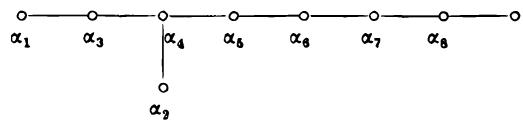
\includegraphics[keepaspectratio]{images/part002_295bff8e.jpg}}

\begin{enumerate}
\def\labelenumi{(\Alph{enumi})}
\setcounter{enumi}{21}
\tightlist
\item
  Since \((\alpha |\alpha) = 2\) for all \(\alpha \in \mathbb{R}\) , we have \(R^{\prime} = R\) .
\end{enumerate}

For \(\Phi_{\mathrm{R}}\) , the squared length of the roots is \(\frac{1}{30}\) ( \(\S 1\) , no. 12). Hence, \(\Phi_{\mathrm{R}}(x,y) = (x|y)/60\) and \(\gamma(\mathrm{R}) = 900\) ( \(\S 1\) , no. 12, formula (20)).

\begin{enumerate}
\def\labelenumi{(\Roman{enumi})}
\setcounter{enumi}{5}
\tightlist
\item
  Calculating the fundamental weights gives
\end{enumerate}

\[
\begin{array}{l} \omega_ {1} = 2 \varepsilon_ {8} = 4 \alpha_ {1} + 5 \alpha_ {2} + 7 \alpha_ {3} + 10 \alpha_ {4} + 8 \alpha_ {5} + 6 \alpha_ {6} + 4 \alpha_ {7} + 2 \alpha_ {8} \\ \omega_ {2} = \frac {1}{2} (\varepsilon_ {1} + \varepsilon_ {2} + \varepsilon_ {3} + \varepsilon_ {4} + \varepsilon_ {5} + \varepsilon_ {6} + \varepsilon_ {7} + 5 \varepsilon_ {8}) \\ \qquad = 5 \alpha_ {1} + 8 \alpha_ {2} + 10 \alpha_ {3} + 15 \alpha_ {4} + 12 \alpha_ {5} + 9 \alpha_ {6} + 6 \alpha_ {7} + 3 \alpha_ {8} \\ \omega_ {3} = \frac {1}{2} (- \varepsilon_ {1} + \varepsilon_ {2} + \varepsilon_ {3} + \varepsilon_ {4} + \varepsilon_ {5} + \varepsilon_ {6} + \varepsilon_ {7} + 7 \varepsilon_ {8}) \\ \qquad = 7 \alpha_ {1} + 10 \alpha_ {2} + 14 \alpha_ {3} + 20 \alpha_ {4} + 16 \alpha_ {5} + 12 \alpha_ {6} + 8 \alpha_ {7} + 4 \alpha_ {8} \\ \omega_ {4} = \varepsilon_ {3} + \varepsilon_ {4} + \varepsilon_ {5} + \varepsilon_ {6} + \varepsilon_ {7} + 5 \varepsilon_ {8} \\ \qquad = 10 \alpha_ {1} + 15 \alpha_ {2} + 20 \alpha_ {3} + 30 \alpha_ {4} + 24 \alpha_ {5} + 18 \alpha_ {6} + 12 \alpha_ {7} + 6 \alpha_ {8} \\ \omega_ {5} = \varepsilon_ {4} + \varepsilon_ {5} + \varepsilon_ {6} + \varepsilon_ {7} + 4 \varepsilon_ {8} \\ \qquad = 8 \alpha_ {1} + 12 \alpha_ {2} + 16 \alpha_ {3} + 24 \alpha_ {4} + 20 \alpha_ {5} + 15 \alpha_ {6} + 10 \alpha_ {7} + 5 \alpha_ {8} \\ \omega_ {6} = \varepsilon_ {5} + \varepsilon_ {6} + \varepsilon_ {7} + 3 \varepsilon_ {8} \\ \qquad = 6 \alpha_ {1} + 9 \alpha_ {2} + 12 \alpha_ {3} + 18 \alpha_ {4} + 15 \alpha_ {5} + 12 \alpha_ {6} + 8 \alpha_ {7} + 4 \alpha_ {8} \\ \omega_ {7} = \varepsilon_ {6} + \varepsilon_ {7} + 2 \varepsilon_ {8} \\ \qquad = 4 \alpha_ {1} + 6 \alpha_ {2} + 8 \alpha_ {3} + 2 \alpha_ {4} + 10 \alpha_ {5} + 8 \alpha_ {6} + 6 \alpha_ {7} + 3 \alpha_ {8} \\ \omega_ {8} = \varepsilon_ {7} + \varepsilon_ {8} \\ \qquad = 5 \alpha_ {1} + 8 \alpha_ {2} + 10 \alpha_ {3} + 15 \alpha_ {4} + 12 \alpha_ {5} + 9 \alpha_ {6} + 6 \alpha_ {7} + 3 \alpha_ {8} = \tilde {\alpha}. \end{array}
\]

\begin{enumerate}
\def\labelenumi{(\Roman{enumi})}
\setcounter{enumi}{6}
\tightlist
\item
  Half the sum of the positive roots is the sum of the fundamental weights (§ 1, no. 10, Prop. 29); this gives
\end{enumerate}

\[
\begin{array}{r l} \rho & = \varepsilon_ {2} + 2 \varepsilon_ {3} + 3 \varepsilon_ {4} + 4 \varepsilon_ {5} + 5 \varepsilon_ {6} + 6 \varepsilon_ {7} + 23 \varepsilon_ {8} \\ & = 46 \alpha_ {1} + 68 \alpha_ {2} + 91 \alpha_ {3} + 135 \alpha_ {4} + 110 \alpha_ {5} + 84 \alpha_ {6} + 57 \alpha_ {7} + 29 \alpha_ {8}. \end{array}
\]

\begin{enumerate}
\def\labelenumi{(\Roman{enumi})}
\setcounter{enumi}{7}
\item
  The group \(Q(R)\) is generated by the \(\varepsilon_{i} \pm \varepsilon_{j}\) and \(\frac{1}{2} \sum_{i=1}^{8} \varepsilon_{i}\) , and is equal to \(L_{3}\) (no. 4). Hence \(P(R)\) , which is associated to \(Q(R^{\prime}) = Q(R) = L_{3}\) , is \(L_{3}\) (no. 4). The connection index is 1.
\item
  The family of exponents has 8 terms, and since h = 30, the integers 1, 7, 11, 13, 17, 19, 23, 29, coprime to 30, must feature in this family; consequently, these are the exponents of W(R).
\item
  From (IX) and Chap. V, § 6, no. 2, Cor. 1 of Prop. 3, it follows that the order of W(R) is
\end{enumerate}

\[
2. 8. 12. 14. 18. 20. 24. 30 = 2 ^ {14}. 3 ^ {5}. 5 ^ {2}. 7.
\]

\begin{enumerate}
\def\labelenumi{(\Roman{enumi})}
\setcounter{enumi}{10}
\tightlist
\item
  The only automorphism of the Dynkin graph is the identity since the three chains issuing from the ramification point have distinct lengths. Hence, \(A(R) = W(R)\) and \(w_{0} = -1\) .
\end{enumerate}

\subsection{\texorpdfstring{SYSTEM OF TYPE \(E_{7}\)}{SYSTEM OF TYPE E\_7}}

\begin{enumerate}
\def\labelenumi{(\Roman{enumi})}
\tightlist
\item
  and (II) Let \(E = R^{8}\) , and let \(R_{8}\) be the root system in E constructed in no. 10. Let V be the hyperplane in E generated by the roots \(\alpha_{1}, \ldots, \alpha_{7}\) of \(R_{8}\) ; it is orthogonal to the eighth fundamental weight \(\omega = \varepsilon_{7} + \varepsilon_{8}\) of \(R_{8}\) .
\end{enumerate}

Let \(R = R_{8} \cap V\) . Then \(R\) is a reduced root system with basis \((\alpha_{1}, \ldots, \alpha_{7})\) , cf.~§ 1. no. 7, Cor. 4 of Prop. 20; hence, this system is of type \(E_{7}\) . Its elements are:

\[
\begin{array}{c} \pm \varepsilon_ {i} \pm \varepsilon_ {j} (1 \leqslant i < j \leqslant 6), \quad \pm (\varepsilon_ {7} - \varepsilon_ {8}), \\ \pm \frac {1}{2} (\varepsilon_ {7} - \varepsilon_ {8} + \sum_ {i = 1} ^ {8} (- 1) ^ {\nu (i)} \varepsilon_ {i}) \quad \text { with } \sum_ {i = 1} ^ {8} \nu (i) \text { odd }. \end{array}
\]

The number of roots is \(n = 2 + \binom{6}{2}.4 + 2^6 = 126\) . The positive roots are

\[
\pm \varepsilon_ {i} + \varepsilon_ {j} (1 \leqslant i <   j \leqslant 6). - \varepsilon_ {7} + \varepsilon_ {8},
\]

\[
\frac {1}{2} \left(- \varepsilon_ {7} + \varepsilon_ {8} + \sum_ {i = 1} ^ {6} (- 1) ^ {\nu (i)} \varepsilon_ {i}\right) \quad \text { with } \sum_ {i = 1} ^ {6} \nu (i) \text { odd }.
\]

\begin{enumerate}
\def\labelenumi{(\Roman{enumi})}
\setcounter{enumi}{2}
\item
  We have \(h = \frac{n}{l} = 18\) .
\item
  Let \(\tilde{\alpha} = \varepsilon_8 - \varepsilon_7 = 2\alpha_1 + 2\alpha_2 + 3\alpha_3 + 4\alpha_4 + 3\alpha_5 + 2\alpha_6 + \alpha_7\) , which is a root. The sum of its coordinates with respect to \((\alpha_i)\) is \(17 = h - 1\) . It is therefore the highest root. It is orthogonal to \(\alpha_i\) for \(2 \leqslant i \leqslant 7\) , and \((\tilde{\alpha}|\alpha_1) = 1\) . The completed Dynkin graph is
\end{enumerate}

\pandocbounded{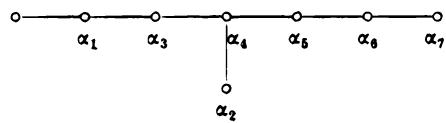
\includegraphics[keepaspectratio]{images/part002_8927380c.jpg}}

\begin{enumerate}
\def\labelenumi{(\Alph{enumi})}
\setcounter{enumi}{21}
\tightlist
\item
  Since \((\alpha |\alpha) = 2\) for all \(\alpha \in \mathbb{R}\) , we have \(R^{\prime} = R\) .
\end{enumerate}

For \(\Phi_{\mathrm{R}}\) , the squared length of the roots is \(\frac{1}{18}\) , so

\[
\Phi_ {\mathrm{R}} (x, y) = (x | y) / 36, \quad \text { and } \quad \gamma (\mathrm{R}) = 2 ^ {2}. 3 ^ {4}
\]

(§ 1. no. 12, formula (20)).

\begin{enumerate}
\def\labelenumi{(\Roman{enumi})}
\setcounter{enumi}{5}
\tightlist
\item
  Calculating the fundamental weights gives
\end{enumerate}

\[
\begin{array}{r l} & {\omega_ {1} = \varepsilon_ {8} - \varepsilon_ {7} = 2 \alpha_ {1} + 2 \alpha_ {2} + 3 \alpha_ {3} + 4 \alpha_ {4} + 3 \alpha_ {5} + 2 \alpha_ {6} + \alpha_ {7}} \\ & {\omega_ {2} = \frac {1}{2} (\varepsilon_ {1} + \varepsilon_ {2} + \varepsilon_ {3} + \varepsilon_ {4} + \varepsilon_ {5} + \varepsilon_ {6} - 2 \varepsilon_ {7} + 2 \varepsilon_ {8})} \\ & {\qquad = \frac {1}{2} (4 \alpha_ {1} + 7 \alpha_ {2} + 8 \alpha_ {3} + 12 \alpha_ {4} + 9 \alpha_ {5} + 8 \alpha_ {6} + 3 \alpha_ {7})} \\ & {\omega_ {3} = \frac {1}{2} (- \varepsilon_ {1} + \varepsilon_ {2} + \varepsilon_ {3} + \varepsilon_ {4} + \varepsilon_ {5} + \varepsilon_ {6} - 3 \varepsilon_ {7} + 3 \varepsilon_ {8})} \\ & {\qquad = 3 \alpha_ {1} + 4 \alpha_ {2} + 6 \alpha_ {3} + 8 \alpha_ {4} + 6 \alpha_ {5} + 4 \alpha_ {6} + 2 \alpha_ {7}} \\ & {\omega_ {4} = \varepsilon_ {3} + \varepsilon_ {4} + \varepsilon_ {5} + \varepsilon_ {6} + 2 (\varepsilon_ {8} - \varepsilon_ {7})} \\ & {\qquad = 4 \alpha_ {1} + 6 \alpha_ {2} + 8 \alpha_ {3} + 12 \alpha_ {4} + 9 \alpha_ {5} + 6 \alpha_ {6} + 3 \alpha_ {7}} \\ & {\omega_ {5} = \varepsilon_ {4} + \varepsilon_ {5} + \varepsilon_ {6} + \frac {3}{2} (\varepsilon_ {8} - \varepsilon_ {7})} \\ & {\qquad = \frac {1}{2} (6 \alpha_ {1} + 9 \alpha_ {2} + 12 \alpha_ {3} + 18 \alpha_ {4} + 15 \alpha_ {5} + 10 \alpha_ {6} + 5 \alpha_ {7})} \\ & {\omega_ {6} = \varepsilon_ {5} + \varepsilon_ {6} - \varepsilon_ {7} + \varepsilon_ {8}} \\ & {\qquad = 2 \alpha_ {1} + 3 \alpha_ {2} + 4 \alpha_ {3} + 6 \alpha_ {4} + 5 \alpha_ {5} + 4 \alpha_ {6} + 2 \alpha_ {7}} \\ & {\omega_ {7} = \varepsilon_ {6} + \frac {1}{2} (\varepsilon_ {8} - \varepsilon_ {7})} \\ & {\qquad = \frac {1}{2} (2 \alpha_ {1} + 3 \alpha_ {2} + 4 \alpha_ {3} + 6 \alpha_ {4} + 5 \alpha_ {5} + 4 \alpha_ {6} + 3 \alpha_ {7}).} \end{array}
\]

\begin{enumerate}
\def\labelenumi{(\Roman{enumi})}
\setcounter{enumi}{6}
\tightlist
\item
  The sum \(2\rho\) of the positive roots is \(2\sum_{i=1}^{7}\omega_i\) (§ 1. no. 10. Prop. 29), so
\end{enumerate}

\[
\begin{array}{r l} 2 \rho & = 2 \varepsilon_ {2} + 4 \varepsilon_ {3} + 6 \varepsilon_ {4} + 8 \varepsilon_ {5} + 10 \varepsilon_ {6} - 17 \varepsilon_ {7} + 17 \varepsilon_ {8} \\ & = 34 \alpha_ {1} + 49 \alpha_ {2} + 66 \alpha_ {3} + 96 \alpha_ {4} + 75 \alpha_ {5} + 52 \alpha_ {6} + 27 \alpha_ {7}. \end{array}
\]

\begin{enumerate}
\def\labelenumi{(\Roman{enumi})}
\setcounter{enumi}{7}
\tightlist
\item
  By no. 10 (VIII) and § 1, no. 10. Prop. 28, we have
\end{enumerate}

\[
\mathrm{Q} (\mathrm{R}) = \mathrm{Q} (\mathrm{R} _ {8}) \cap \mathrm{V} = \mathrm{L} _ {3} \cap \mathrm{V} \quad \text { and } \quad \mathrm{P} (\mathrm{R}) = p (\mathrm{P} (\mathrm{R} _ {8})) = p (\mathrm{L} _ {3}),
\]

where p denotes the orthogonal projection of E onto V. The group \(Q(R)\) has basis \((\alpha_{1},\ldots,\alpha_{7})\) : the group \(P(R)\) is generated by \(Q(R)\) and

\[
p (\alpha_ {8}) = \alpha_ {8} - \frac {1}{2} \omega .
\]

We have \(\omega\in\mathrm{P}(\mathrm{R}_{8})\) , \(\frac{1}{2}\omega\notin\mathrm{P}(\mathrm{R}_{8})\) , so \(2p(\alpha_{8})\in\mathrm{Q}(\mathrm{R})\) and \(p(\alpha_{8})\notin\mathrm{Q}(\mathrm{R})\) . Thus, \(\mathrm{P}(\mathrm{R})/\mathrm{Q}(\mathrm{R})\) is isomorphic to Z/2Z and is generated by, for example, the image of \(\omega_{7}\) .

The connection index is 2.

\begin{enumerate}
\def\labelenumi{(\Roman{enumi})}
\setcounter{enumi}{8}
\tightlist
\item
  The sequence of exponents of \(W(R)\) has 7 terms. The numbers 1, 5, 7, 11, 13, 17, coprime to \(h = 18\) , feature in this sequence. The last exponent \(m\) must be such that \(m + m = 18\) (Chap. V, § 6. no. 2, formula (2)). Hence, the sequence of exponents is
\end{enumerate}

\[
1, 5, 7, 9, 11, 13, 17.
\]

\begin{enumerate}
\def\labelenumi{(\Alph{enumi})}
\setcounter{enumi}{23}
\tightlist
\item
  From (IX) and Chap. V. § 6, no. 2, Cor. 1 of Prop. 3, it follows that the order of W(R) is
\end{enumerate}

\[
2. 6. 8. 10. 12. 14. 18 = 2 ^ {10}. 3 ^ {4}. 5. 7.
\]

\begin{enumerate}
\def\labelenumi{(\Roman{enumi})}
\setcounter{enumi}{10}
\item
  The only automorphism of the Dynkin graph is the identity, so \(\mathbf{A}(\mathbf{R}) = \mathbf{W}(\mathbf{R})\) and \(w_0 = -1\) .
\item
  \(\mathrm{P}(\mathrm{R}^{-})/\mathrm{Q}(\mathrm{R}^{-})\) has only one non-identity element. It interchanges the vertices corresponding to \(\alpha_{0}\) and \(\alpha_{7}\) , \(\alpha_{1}\) and \(\alpha_{6}\) , \(\alpha_{3}\) and \(\alpha_{5}\) , and leaves \(\alpha_{2}\) and \(\alpha_{4}\) fixed.
\end{enumerate}

\subsection{\texorpdfstring{SYSTEM OF TYPE \(E_{6}\)}{SYSTEM OF TYPE E\_6}}

\begin{enumerate}
\def\labelenumi{(\Roman{enumi})}
\tightlist
\item
  and (II) Let \(E = R^{8}\) , and let \(R_{8}\) be the root system in E constructed in no. 10. Let V be the vector subspace of E generated by the roots \(\alpha_{1}, \ldots, \alpha_{6}\) of \(R_{8}\) ; this is the orthogonal complement of the plane generated by the last two fundamental weights \(\omega = \varepsilon_{7} + \varepsilon_{8}\) and \(\pi = \varepsilon_{6} + \varepsilon_{7} + 2\varepsilon_{8}\) of \(R_{8}\) .
\end{enumerate}

Let \(R = R_{8} \cap V\) . This is a reduced root system with basis \((\alpha_{1}, \ldots, \alpha_{6})\) , and hence of type \(E_{6}\) . Its elements are:

\[
\begin{array}{c} \pm \varepsilon_ {i} \pm \varepsilon_ {j} (1 \leqslant i <   j \leqslant 5), \\ \pm \frac {1}{2} (\varepsilon_ {8} - \varepsilon_ {7} - \varepsilon_ {6} + \sum_ {i = 1} ^ {5} (- 1) ^ {\nu (i)} \varepsilon_ {i}) \text {with} \sum_ {i = 1} ^ {5} \nu (i) \text {even.} \end{array}
\]

The number of roots is \(n = \binom{5}{2}.4 + 2^5 = 72\) . The positive roots are

\[
\pm \varepsilon_ {i} + \varepsilon_ {j} (1 \leqslant i <   j \leqslant 5),
\]

\[
\frac {1}{2} \left(\varepsilon_ {8} - \varepsilon_ {7} - \varepsilon_ {6} + \sum_ {i = 1} ^ {5} (- 1) ^ {\nu (i)} \varepsilon_ {i}\right) \text {with} \sum_ {i = 1} ^ {5} \nu (i) \text {even}.
\]

\begin{enumerate}
\def\labelenumi{(\Roman{enumi})}
\setcounter{enumi}{2}
\item
  We have \(h = \frac{n}{6} = 12\) .
\item
  Let
\end{enumerate}

\[
\begin{array}{r l} \tilde {\alpha} & = \frac {1}{2} (\varepsilon_ {1} + \varepsilon_ {2} + \varepsilon_ {3} + \varepsilon_ {4} + \varepsilon_ {5} - \varepsilon_ {6} - \varepsilon_ {7} + \varepsilon_ {8}) \\ & = \alpha_ {1} + 2 \alpha_ {2} + 2 \alpha_ {3} + 3 \alpha_ {4} + 2 \alpha_ {5} + \alpha_ {6}, \end{array}
\]

which is a root. The sum of its coordinates with respect to \((\alpha_{i})\) is 11 = h - 1, so \(\tilde{\alpha}\) is the highest root. It is orthogonal to \(\alpha_{1}, \alpha_{3}, \alpha_{4}, \alpha_{5}, \alpha_{6}\) , and \((\tilde{\alpha}|\alpha_{2}) = 1\) . The completed Dynkin graph is

\pandocbounded{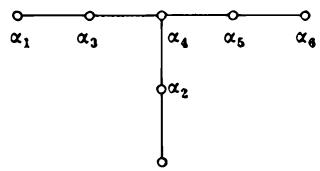
\includegraphics[keepaspectratio]{images/part002_9f0044a9.jpg}}

\begin{enumerate}
\def\labelenumi{(\Alph{enumi})}
\setcounter{enumi}{21}
\tightlist
\item
  Since \((\alpha |\alpha) = 2\) for all \(\alpha \in \mathbb{R}\) , we have \(\mathbb{R}^{\sim} = \mathbb{R}\) . For \(\Phi_{\mathbb{R}}\) , the squared length of the roots is \(\frac{1}{12}\) , so
\end{enumerate}

\[
\Phi_ {\mathrm{R}} (x, y) = (x | y) / 24, \quad \text { and } \quad \gamma (\mathrm{R}) = 144.
\]

\begin{enumerate}
\def\labelenumi{(\Roman{enumi})}
\setcounter{enumi}{5}
\tightlist
\item
  Calculating the fundamental weights gives:
\end{enumerate}

\[
\begin{array}{l} \omega_ {1} = \frac {2}{3} (\varepsilon_ {8} - \varepsilon_ {7} - \varepsilon_ {6}) = \frac {1}{3} (4 \alpha_ {1} + 3 \alpha_ {2} + 5 \alpha_ {3} + 6 \alpha_ {4} + 4 \alpha_ {5} + 2 \alpha_ {6}) \\ \omega_ {2} = \frac {1}{2} (\varepsilon_ {1} + \varepsilon_ {2} + \varepsilon_ {3} + \varepsilon_ {4} + \varepsilon_ {5} - \varepsilon_ {6} - \varepsilon_ {7} + \varepsilon_ {8}) \\ \quad = \alpha_ {1} + 2 \alpha_ {2} + 2 \alpha_ {3} + 3 \alpha_ {4} + 2 \alpha_ {5} + \alpha_ {6} = \tilde {\alpha} \\ \omega_ {3} = \frac {5}{6} (\varepsilon_ {8} - \varepsilon_ {7} - \varepsilon_ {6}) + \frac {1}{2} (- \varepsilon_ {1} + \varepsilon_ {2} + \varepsilon_ {3} + \varepsilon_ {4} + \varepsilon_ {5}) \\ \quad = \frac {1}{3} (5 \alpha_ {1} + 6 \alpha_ {2} + 10 \alpha_ {3} + 12 \alpha_ {4} + 8 \alpha_ {5} + 4 \alpha_ {6}) \\ \omega_ {4} = \varepsilon_ {3} + \varepsilon_ {4} + \varepsilon_ {5} - \varepsilon_ {6} - \varepsilon_ {7} + \varepsilon_ {8} \\ \quad = 2 \alpha_ {1} + 3 \alpha_ {2} + 4 \alpha_ {3} + 6 \alpha_ {4} + 4 \alpha_ {5} + 2 \alpha_ {6} \\ \omega_ {5} = \frac {2}{3} (\varepsilon_ {8} - \varepsilon_ {7} - \varepsilon_ {6}) + \varepsilon_ {4} + \varepsilon_ {5} \\ \quad = \frac {1}{3} (4 \alpha_ {1} + 6 \alpha_ {2} + 8 \alpha_ {3} + 12 \alpha_ {4} + 10 \alpha_ {5} + 5 \alpha_ {6}) \\ \omega_ {6} = \frac {1}{3} (\varepsilon_ {8} - \varepsilon_ {7} - \varepsilon_ {6}) + \varepsilon_ {5} \\ \quad = \frac {1}{3} (2 \alpha_ {1} + 3 \alpha_ {2} + 4 \alpha_ {3} + 6 \alpha_ {4} + 5 \alpha_ {5} + 4 \alpha_ {6}). \end{array}
\]

\begin{enumerate}
\def\labelenumi{(\Roman{enumi})}
\setcounter{enumi}{6}
\tightlist
\item
  Half the sum of the positive roots is \(\sum_{i=1}^{6} \omega_i\) , so
\end{enumerate}

\[
\begin{array}{r l} \rho & = \varepsilon_ {2} + 2 \varepsilon_ {3} + 3 \varepsilon_ {4} + 4 \varepsilon_ {5} + 4 (\varepsilon_ {8} - \varepsilon_ {7} - \varepsilon_ {6}) \\ & = 8 \alpha_ {1} + 11 \alpha_ {2} + 15 \alpha_ {3} + 21 \alpha_ {4} + 15 \alpha_ {5} + 8 \alpha_ {6}. \end{array}
\]

\begin{enumerate}
\def\labelenumi{(\Roman{enumi})}
\setcounter{enumi}{7}
\tightlist
\item
  By no. 10 (VIII) and § 1, no. 10, Prop. 28,
\end{enumerate}

\[
\mathrm{Q} (\mathrm{R}) = \mathrm{Q} (\mathrm{R} _ {8}) \cap \mathrm{V} = \mathrm{L} _ {3} \cap \mathrm{V} \quad \text { and } \quad \mathrm{P} (\mathrm{R}) = p (\mathrm{P} (\mathrm{R} _ {8})) = p (\mathrm{L} _ {3}),
\]

where p denotes the orthogonal projection of E onto V. We have

\[
p (\alpha_ {7}) = \alpha_ {7} - \frac {2}{3} \pi + \omega , \quad p (\alpha_ {8}) = \alpha_ {8} + \pi - 2 \omega .
\]

The group \(Q(R)\) has basis \((\alpha_{1},\ldots,\alpha_{6})\) . The group \(P(R)\) is generated by \(Q(R)\) and \(p(\alpha_{7})\) , since \(p(\alpha_{8})\in P(R_{8})\cap V=Q(R_{8})\cap V=Q(R)\) . We have \(3p(\alpha_{7})\in Q(R)\) and \(p(\alpha_{7})\notin Q(R)\) . Hence, the group \(P(R)/Q(R)\) is isomorphic to Z/3Z; it is generated, for example, by the image of \(\omega_{6}\) .

The connection index is 3.

\begin{enumerate}
\def\labelenumi{(\Roman{enumi})}
\setcounter{enumi}{8}
\tightlist
\item
  (IX) and (X) By § 2. no. 4. Prop. 7, the order of the Weyl group is 6!1.2.2.3.2.1.3 = \(2^{7}.3^{4}.5\) . The sequence of exponents has 6 terms between 1 and 11, and contains the integers 1, 5, 7, 11 which are coprime to 12. The other exponents \(m, m'\) are integers such that
\end{enumerate}

\[
m + m ^ {\prime} = 12.
\]

\[
(m + 1) \left(m ^ {\prime} + 1\right) (1 + 1) (5 + 1) (7 + 1) (11 + 1) = 2 ^ {7}. 3 ^ {4}. 5,
\]

in view of Chap. V. § 6, no. 2, formula (2) and Cor. 1 of Prop. 3. The second relation gives \((m + 1)(m' + 1) = 45\) , and since \(m + m' + 2 = 14\) , we obtain \(m = 4\) , \(m' = 8\) . Hence, the sequence of exponents is

\[
1, 4, 5, 7, 8, 11.
\]

\begin{enumerate}
\def\labelenumi{(\Roman{enumi})}
\setcounter{enumi}{10}
\tightlist
\item
  (XI) and (XII) Since the roots all have the same length, the automorphisms of the Dynkin graph are those of the underlying graph. Apart from the identity, there is only the automorphism \(\varepsilon\) which transforms \(\alpha_{1},\alpha_{3},\alpha_{4},\alpha_{5},\alpha_{6},\) \(\alpha_{2}\) into \(\alpha_{6},\alpha_{5},\alpha_{4},\alpha_{3},\alpha_{1},\alpha_{2}\) , respectively. Hence, \(\mathrm{A(R) / W(R)}\) is isomorphic to \(\mathbf{Z} / 2\mathbf{Z}\) ; since \(-1\in \mathrm{W(R)}\) (Chap. V. §6, no. 2, Cor. 3 of Prop. 3), \(\mathrm{A(R)}\) is isomorphic to \(\mathrm{W(R)}\times \{1, - 1\}\) and \(w_0\) can be identified with \(-\varepsilon\) . It follows that the non-identity element of \(\mathrm{A(R) / W(R)}\) defines the automorphism \(x\mapsto -x\) of \(\mathrm{P(R^{\prime}) / Q(R^{\prime})}\) .
\end{enumerate}

Moreover, \(P(R^{-})/Q(R^{-})\) has two non-identity elements of order 3. They define the two automorphisms of order 3 of the completed Dynkin graph.

\subsection{\texorpdfstring{SYSTEM OF TYPE \(G_{2}\)}{SYSTEM OF TYPE G\_2}}

\begin{enumerate}
\def\labelenumi{(\Roman{enumi})}
\tightlist
\item
  Let E be the hyperplane in \(R^{3}\) with equation
\end{enumerate}

\[
\xi_ {1} + \xi_ {2} + \xi_ {3} = 0.
\]

Let \(R\) be the set of \(\alpha \in L_0 \cap V\) such that \((\alpha | \alpha) = 2\) or \((\alpha | \alpha) = 6\) . The elements of \(R\) are

\[
\begin{array}{c} \pm (\varepsilon_ {1} - \varepsilon_ {2}), \quad \pm (\varepsilon_ {1} - \varepsilon_ {3}), \quad \pm (\varepsilon_ {2} - \varepsilon_ {3}), \quad \pm (2 \varepsilon_ {1} - \varepsilon_ {2} - \varepsilon_ {3}), \\ \pm (2 \varepsilon_ {2} - \varepsilon_ {1} - \varepsilon_ {3}), \quad \pm (2 \varepsilon_ {3} - \varepsilon_ {1} - \varepsilon_ {2}). \end{array}
\]

Then, R generates V, and \(\frac{2(\alpha|\beta)}{(\beta|\beta)}\in\mathbf{Z}\) for all \(\alpha,\beta\in R\) : this is clear if \(\beta=\pm(\varepsilon_{i}-\varepsilon_{j})\) with \(i\neq j\) ; if \(\beta=2\varepsilon_{1}-\varepsilon_{2}-\varepsilon_{3}\) for example, we have \((\alpha|\beta)\in3\mathbf{Z}\) , and again our assertion holds. Hence, R is a reduced root system in V. The number of roots is n=12.

\begin{enumerate}
\def\labelenumi{(\Roman{enumi})}
\setcounter{enumi}{1}
\tightlist
\item
  Put \(\alpha_{1} = \varepsilon_{1} - \varepsilon_{2},\alpha_{2} = -2\varepsilon_{1} + \varepsilon_{2} + \varepsilon_{3}\) . Then the roots are
\end{enumerate}

\[
\begin{array}{r l} & {\pm \alpha_ {1}, \quad \pm (\alpha_ {1} + \alpha_ {2}), \quad \pm (2 \alpha_ {1} + \alpha_ {2}), \quad \pm \alpha_ {2},} \\ & {\qquad \pm (3 \alpha_ {1} + \alpha_ {2}), \quad \pm (3 \alpha_ {1} + 2 \alpha_ {2}).} \end{array}
\]

Hence, \((\alpha_{1},\alpha_{2})\) is a basis of \(R\) . We have \(\| \alpha_{1}\|^{2} = 2,\| \alpha_{2}\|^{2} = 6.\) \((\alpha_{1}|\alpha_{2}) = -3,\) so \(R\) is a system of type \(G_{2}\) . The positive roots are \(\alpha_{1},\alpha_{1} + \alpha_{2},2\alpha_{1} + \alpha_{2},\) \(3\alpha_{1} + \alpha_{2},3\alpha_{1} + 2\alpha_{2}\) .

\begin{enumerate}
\def\labelenumi{(\Roman{enumi})}
\setcounter{enumi}{2}
\item
  We have \(h = \frac{n}{2} = 6\) .
\item
  The highest root is \(\tilde{\alpha} = 3\alpha_{1} + 2\alpha_{2} = -\varepsilon_{1} - \varepsilon_{2} + 2\varepsilon_{3}\) . We have \((\tilde{\alpha}|\alpha_{1}) = 0, (\tilde{\alpha}|\alpha_{2}) = 3\) . The completed Dynkin graph is
\end{enumerate}

\[
\alpha_ {1} \quad \alpha_ {2}
\]

\begin{enumerate}
\def\labelenumi{(\Alph{enumi})}
\setcounter{enumi}{21}
\tightlist
\item
  The inverse system is the following set of vectors:
\end{enumerate}

\[
\begin{array}{l} \pm \alpha_ {1}, \quad \pm (\alpha_ {1} + \alpha_ {2}), \quad \pm (2 \alpha_ {1} + \alpha_ {2}), \quad \pm \frac {1}{3} \alpha_ {2}, \\ \qquad \pm \frac {1}{3} (3 \alpha_ {1} + \alpha_ {2}), \quad \pm \frac {1}{3} (3 \alpha_ {1} + 2 \alpha_ {2}). \end{array}
\]

There are 10 roots not orthogonal to \(\alpha_{1}\) ; we have \(n(\beta, \alpha_{1}) = \pm 1\) for 4 of these roots, \(n(\beta, \alpha_{1}) = \pm 3\) for 4 others, and \(n(\beta, \alpha_{1}) = \pm 2\) for \(\beta = \pm \alpha_{1}\) . Hence, the squared length of \(\alpha_{1}\) for \(\Phi_{\mathbb{R}}\) is \(4(4.1 + 4.9 + 2.4)^{-1} = \frac{1}{12}\) . Hence, \(\Phi_{\mathbb{R}}(x, y) = (x|y)/24\) . We now apply formula (18) of §1, no. 12, with \(x = y = \alpha_{1}\) ; this gives

\[
2 + 4. \frac {1}{4} + 4. \frac {1}{4} = \gamma (\mathrm{R}). \frac {1}{12}
\]

so \(\gamma (\mathbb{R}) = 48\)

\begin{enumerate}
\def\labelenumi{(\Roman{enumi})}
\setcounter{enumi}{5}
\tightlist
\item
  (VI) and (VII) Half the sum of the positive roots is
\end{enumerate}

\[
\rho = 5 \alpha_ {1} + 3 \alpha_ {2}.
\]

The fundamental weights \(\omega_{1}\) and \(\omega_{2}\) are orthogonal to \(\alpha_{2}\) and \(\alpha_{1}\) , hence proportional to \(2\alpha_{1} + \alpha_{2}\) and \(3\alpha_{1} + 2\alpha_{2}\) . We have

\[
\omega_ {1} + \omega_ {2} = \rho = 5 \alpha_ {1} + 3 \alpha_ {2} = (2 \alpha_ {1} + \alpha_ {2}) + (3 \alpha_ {1} + 2 \alpha_ {2}).
\]

Hence,

\[
\omega_ {1} = 2 \alpha_ {1} + \alpha_ {2}, \quad \omega_ {2} = 3 \alpha_ {1} + 2 \alpha_ {2} = \tilde {\alpha}.
\]

\begin{enumerate}
\def\labelenumi{(\Roman{enumi})}
\setcounter{enumi}{7}
\item
  Q(R) is generated by \(\varepsilon_{1}-\varepsilon_{2}\) and \(\varepsilon_{1}-\varepsilon_{3}\) , for example. By (VI) and (VII), P(R) = Q(R). The connection index is 1.
\item
  The family of exponents has 2 terms: since 1 and \(h - 1 = 5\) are exponents, they are the only ones.
\item
  We have \((\alpha_{1},\alpha_{2}) = \frac{5\pi}{6}\) , so \(\mathrm{W}(\mathbb{R})\) is isomorphic to the dihedral group of order 12.
\item
  The only automorphism of the Dynkin diagram is the identity, so \(A(R) = W(R)\) and \(w_{0} = -1\) .
\end{enumerate}

\subsection{IRREDUCIBLE NON-REDUCED ROOT SYSTEMS}

The irreducible, non-reduced root systems can be obtained from the irreducible, reduced systems by using Props. 13 and 14 of §1. no. 4. For each integer \(l \geqslant 1\) , there exists, up to isomorphism, a unique irreducible. non-reduced root system of rank \(l\) : let \(R\) be a root system of type \(B_l\) . A the set of shortest roots of \(R\) ; take the union of \(R\) and \(2A\) . With the notation of no. 5, we obtain the \(2l(l + 1)\) vectors

\[
\pm \varepsilon_ {i}, \quad \pm 2 \varepsilon_ {i}, \quad \varepsilon_ {i} \pm \varepsilon_ {j} (i <   j).
\]

\exercisesection{Exercises for § 1}

All the root systems considered below are relative to real vector spaces. We denote by \((x|y)\) a scalar product invariant under the Weyl group (cf.~no. 3).

\begin{enumerate}
\def\labelenumi{\arabic{enumi})}
\item
  Let \(\mathbb{R}\) be a root system, \(\mathbb{R} = \mathbb{R}_1 \cup \mathbb{R}_2\) a partition of \(\mathbb{R}\) . Assume that, if \(x, y\) are two elements of \(\mathbb{R}_i\) and if \(x + y\) (resp. \(x - y\) ) is a root, then \(x + y \in \mathbb{R}_i\) (resp. \(x - y \in \mathbb{R}_i\) ), where \(i = 1, 2\) . Then, \(\mathbb{R}\) is the direct sum of \(\mathbb{R}_1\) and \(\mathbb{R}_2\) . (By using the Cor. of Th. 1, no. 3, show that if \(x \in \mathbb{R}_1\) and \(y \in \mathbb{R}_2\) then \((x|y) = 0\) .)
\item
  Let R be a root system, \(\alpha\) and \(\beta\) two roots. If t is a scalar such that \(\beta + t\alpha \in R\) , then \(2t \in Z\) . (For \(n(\beta + t\alpha, \alpha) = n(\beta, \alpha) + 2t\) .) If \(\alpha\) is indivisible, then \(t \in Z\) . (If not, show, by using Prop. 9, that there exists a root \(\gamma\) orthogonal to \(\alpha\) such that \(\gamma + \frac{1}{2}\alpha \in R\) : then \((\gamma + \frac{1}{2}\alpha|\alpha) > 0\) , so \(\frac{1}{2}\alpha \in R\) .)
\item
  Let R be an irreducible non-reduced root system in V. There exists a non-degenerate symmetric bilinear form \(\Phi\) on V such that, if we identify V with \(V^{*}\) using \(\Phi\) , we have \(R = R^{-}\) . (Use Prop. 13.)
\item
  Let \(\Gamma\) be a free \(\mathbf{Z}\) -module of finite rank \(l\) , \(\Gamma^{*}\) the dual \(\mathbf{Z}\) -module, I a finite set of indices, \((x_{i}, x_{i}^{*})_{i \in \mathbf{I}}\) a family of elements of \(\Gamma \times \Gamma^{*}\) such that \(\langle x_{i}, x_{i}^{*} \rangle = 2\) for all \(i \in \mathbf{I}\) , \(s_{i} = s_{x_{i}, x_{i}^{*}}\) . Let \(\mathbf{V}\) be the real vector space \(\Gamma \otimes_{\mathbf{Z}} \mathbf{R}\) , whose dual \(\mathbf{V}^{*}\) can be identified with \(\Gamma^{*} \otimes_{\mathbf{Z}} \mathbf{R}\) . We also denote by \(s_{i}\) the reflection \(s_{i} \otimes 1\) in \(\mathbf{V}\) . Let \(\mathbf{R}\) (resp. \(\mathbf{R}'\) ) be the set of \(x_{i}\) (resp. \(x_{i}^{*}\) ). Let \(\mathbf{E}\) (resp. \(\mathbf{E}'\) ) be the subspace of \(\mathbf{V}\) (resp. \(\mathbf{V}^{*}\) ) generated by \(\mathbf{R}\) (resp. \(\mathbf{R}'\) ). Assume that \(s_{i}(\mathbf{R}) = \mathbf{R}\) for all \(i\) . Then, \(\mathbf{R}\) is a root system in \(\mathbf{E}\) . \(\mathbf{E}'\) is canonically identified with the dual of \(\mathbf{E}\) and \(x_{i}^{*}\) with \(x_{i}^{-}\) for all \(i\) . If \(\mathbf{F}\) (resp. \(\mathbf{F}'\)) is the subspace of \(\mathbf{V}\) (resp. \(\mathbf{V}^{*}\) ) consisting of the points invariant under all the \(s_{i}\) (resp. \(^t s_{i}\) ), then \(\Gamma \cap \mathbf{F}\) (resp. \(\Gamma^{*} \cap \mathbf{F}'\) ) generates \(\mathbf{F}\) (resp. \(\mathbf{F}'\) ). If we put \(\Gamma_{1} = (\Gamma \cap \mathbf{E}) \oplus (\Gamma \cap \mathbf{F})\) (resp. \(\Gamma_{1}^{*} = (\Gamma^{*} \cap \mathbf{E}') \oplus (\Gamma^{*} \cap \mathbf{F}')\) ), then \(\Gamma / \Gamma_{1}\) and \(\Gamma^{*} / \Gamma_{1}^{*}\) are isomorphic finite groups.
\item
  Let \(R\) be an irreducible root system. For any \(\beta \in R\) ,
\end{enumerate}

\[
16 \gamma (\mathrm{R}) = (\sum_ {\alpha \in \mathrm{R}} n (\alpha , \beta) ^ {2}) (\sum_ {\alpha \in \mathrm{R}} n (\beta , \alpha) ^ {2})
\]

and consequently \(\gamma (\mathbb{R}) = \gamma (\lambda R)\) for any non-zero scalar \(\lambda\) . (Use formulas (17) and (19) of no. 12.)

\begin{enumerate}
\def\labelenumi{\arabic{enumi})}
\setcounter{enumi}{5}
\tightlist
\item
  \begin{enumerate}
  \def\labelenumii{\alph{enumii})}
  \tightlist
  \item
    Let A be an abelian group of finite type, and T a finite subset of A not containing 0. There exists a subgroup H of A of finite index such that \(H \cap T = \varnothing\) . (Let \(t \in T\) . By using the structure of abelian groups of finite type, construct a subgroup of A of finite index that does not contain t. Now proceed by induction on \(\text{Card}(T)\) .)
  \end{enumerate}
\end{enumerate}

\begin{enumerate}
\def\labelenumi{\alph{enumi})}
\setcounter{enumi}{1}
\tightlist
\item
  Let R be a root system and P a closed symmetric subset of R. There exists a subgroup H of Q(R) of finite index such that \(P = H \cap R\) . (Pass to the quotient by the subgroup of Q(R) generated by P, and use a) and Prop. 23.)
\end{enumerate}

\begin{enumerate}
\def\labelenumi{\arabic{enumi})}
\setcounter{enumi}{6}
\item
  The connection index of a root system is equal to the determinant of its Cartan matrix. (Use formula (14) of no. 10. Show on the other hand that, in a real vector space with a scalar product, if \((\varepsilon_1, \ldots, \varepsilon_n), (\varepsilon_1', \ldots, \varepsilon_n')\) are two bases such that \((\varepsilon_i | \varepsilon_j') = \delta_{ij}\) , then \(\det_{(\varepsilon_1, \ldots, \varepsilon_n)} (\varepsilon_1', \ldots, \varepsilon_n') > 0\) .)
\item
  Let R be a reduced root system, C a chamber, \(2\sigma\) the sum of the positive elements of \(R^{-}\) , \(P'(R)\) the set of \(x \in P(R)\) such that \(\langle x, \sigma \rangle \in Z\) . Then, \(Q(R) \subseteq P'(R) \subseteq P(R)\) , and \(P(R)/P'(R)\) is of order 1 or 2. Let \((\beta_{1}, \ldots, \beta_{l})\) be the basis of \(R^{-}\) corresponding to C, and put \(2\sigma = n_{1}\beta_{1} + \cdots + n_{l}\beta_{l}\) where the \(n_{i}\) are integers \textgreater0. Then, \(P(R) = P'(R)\) if and only if all the \(n_{i}\) are even.
\item
  Let \(\mathbb{R}\) be a root system, \(\mathbb{C}\) a chamber. Put \(\mathrm{B}(\mathbb{C}) = \{\alpha_1, \ldots, \alpha_l\}\) ,
\end{enumerate}

\[
\mathrm{R} _ {+} (\mathrm{C}) = \left\{\alpha_ {1}, \dots , \alpha_ {l}, \alpha_ {l + 1}, \dots , \alpha_ {s} \right\}
\]

(the \(\alpha_{i}\) being pairwise distinct), and \(\alpha = \alpha_{1} + \dots +\alpha_{s}\) .

\begin{enumerate}
\def\labelenumi{\alph{enumi})}
\tightlist
\item
  For \(i = 1, 2, \ldots, s\) , put \(\varepsilon_{i} = \pm 1\) . Let \(\alpha^{*} = \varepsilon_{1}\alpha_{1} + \cdots + \varepsilon_{s}\alpha_{s}\) . If \((\alpha^{*}|\alpha_{i}) > 0\) for \(i = 1, \ldots, l\) , then \(\alpha^{*} = \alpha\) and \(\varepsilon_{i} = 1\) for all i. (Let \(\gamma\) (resp. \(\delta\) ) be the sum of the \(\alpha_{i}\) for which \(\varepsilon_{i} = 1\) (resp. -1). Then, \((\gamma|\alpha_{i}) - (\delta|\alpha_{i}) > 0\) , \((\gamma|\alpha_{i}) + (\delta|\alpha_{i}) = (\alpha_{i}|\alpha_{i})\) , so
\end{enumerate}

\(2(\gamma|\alpha_{i})>(\alpha_{i}|\alpha_{i});\) since \(2(\gamma|\alpha_{i}) / (\alpha_{i}|\alpha_{i})\in \mathbf{Z},(\gamma |\alpha_{i})\geqslant (\alpha_{i}|\alpha_{i}) = (\alpha |\alpha_{i}),\) so \(\gamma -\alpha \in \overline{\mathrm{C}}. \gamma \geqslant \alpha ,\) \(\gamma = \alpha\) and \(\delta = 0.)\)

\begin{enumerate}
\def\labelenumi{\alph{enumi})}
\setcounter{enumi}{1}
\tightlist
\item
  For \(i = 1,2,\ldots,s\) , let \(\varepsilon_{i} = \pm 1\) . The set of \(\varepsilon_{i}\alpha_{i}\) is the set of roots \(>0\) relative to a chamber if and only if \(\alpha^{*} = \sum_{i}\varepsilon_{i}\alpha_{i}\) belongs to a chamber. (To show that the condition is sufficient, let \(\mu_{i} = \pm 1\) be such that \((\alpha^{*}|\mu_{i}\alpha_{i}) > 0\) . There exists an element \(w\in W(R)\) that transforms the set of \(\mu_{i}\alpha_{i}\) into the set of \(\alpha_{i}\) , and hence \(\alpha^{*}\) into \(\alpha^{**} = \sum_{i}\varepsilon_{i}\mu_{i}\alpha_{\sigma(i)}\) , where \(\sigma \in \mathfrak{S}_s\) . Applying \(a\) ), show that \(\alpha^{**} = \alpha\) , so \(\mu_{i}\varepsilon_{i} = 1\) .)
\end{enumerate}

\begin{enumerate}
\def\labelenumi{\arabic{enumi})}
\setcounter{enumi}{9}
\item
  Let \(\alpha\) be the highest root of an irreducible reduced root system R relative to some basis. Then, \(\alpha^{-}\) is the highest root of \(R^{-}\) if and only if all the roots are of the same length.
\item
  With the notation of Prop. 33 of no. 11. show that \(\theta_{i} + \theta_{j}\) is not a root for any pair \((i,j)\) .
\item
  Let R be a root system in V of rank \(\geqslant 3\) , \((\alpha_{1},\ldots,\alpha_{l})\) a basis of R. \(V'\) (resp. \(V''\) ) the subspace of V generated by the \(\alpha_{i}\) for \(i \geqslant 2\) (resp. \(i \geqslant 3\) ). \(R' = R \cap V'\) , \(R'' = R \cap V''\) . Let d (resp. \(d', d''\) ) be the determinant of the Cartan matrix of R (resp. \(R', R''\) ). Assume that \(\alpha_{1}\) is orthogonal to all the \(\alpha_{i}\) except \(\alpha_{2}\) , and that \(\| \alpha_{1} \| = \| \alpha_{2} \|\) . Show that \(d = 2d' - d''\) .
\item
  Let R be a reduced root system. \((\alpha_{1},\ldots,\alpha_{l})\) a basis of R and \(\alpha=c_{1}\alpha_{1}+\cdots+c_{l}\alpha_{l}\) a root. Then, \(c_{i}(\alpha_{i}|\alpha_{i})/(\alpha|\alpha)\in\mathbf{Z}\) for all i. (Consider the inverse system.)
\item
  Let R be an irreducible root system, \(\lambda\) the greatest root length. S the set of subsets of R consisting of pairwise orthogonal roots of length \(\lambda\) . Then, any two maximal elements of S are transformed into each other by W(R). (Use Prop. 11. and Prop. 1 of Chap. V. §3. no. 3.)
\item
  Let \(R\) be a root system of rank \(l\) .
\end{enumerate}

\begin{enumerate}
\def\labelenumi{\alph{enumi})}
\item
  \(-1 \in \mathrm{W}(\mathrm{R})\) if and only if R contains l roots that are pairwise strongly orthogonal. (To show that the condition is necessary, argue by induction on l using Prop. 1 of Chap. V, §3, no. 3.)
\item
  If \(w \in \mathrm{W}(\mathrm{R})\) is of order 2, there exists a set S of pairwise strongly orthogonal roots such that w is the product of the \(s_{\alpha} (\alpha \in \mathrm{S})\) .
\end{enumerate}

\begin{enumerate}
\def\labelenumi{\arabic{enumi})}
\setcounter{enumi}{15}
\tightlist
\item
  Let \(\mathbb{R}\) be a root system. B a basis of \(\mathbb{R}\) , and \(\mathbb{R}_+\) the set of positive roots relative to this basis. For \(w \in W(\mathbb{R})\) , put \(F_w = R_+ \cap w(-R_+)\) . Show that the map \(w \mapsto F_w\) is a bijection from \(W(\mathbb{R})\) to the set of subsets \(F\) of \(R_+\) such that \(F\) and \(R_+ - F\) are closed. (Apply Cor. 1 of Prop. 20 to the subset \(P = (R_+ - F) \cup (-F)\) .)
\end{enumerate}

¶ 17) Let R be a reduced root system and B a basis of R. For any subset J of B, let W \(_{J}\) be the subgroup of W(R) generated by the reflections s \(_{\alpha}\) for \(\alpha \in J\) , and let w \(_{J}\) be the longest element of W \(_{J}\) . Let \(\Phi\) be the set of w \(_{J}\) .

\begin{enumerate}
\def\labelenumi{\alph{enumi})}
\tightlist
\item
  Show that an element \(w \in \mathrm{W}(\mathbb{R})\) belongs to \(\Phi\) if and only if
\end{enumerate}

\[
\mathrm{W} (\mathrm{B}) \subseteq \mathrm{R} _ {+} (\mathrm{B}) \cup (- \mathrm{B}).
\]

(To show that the condition is sufficient. denote by \(\mathrm{J}_1\) the set of \(\alpha \in \mathrm{B}\) such that \(w(\alpha) \in -\mathrm{B}\) and put \(\mathrm{J} = -w(\mathrm{J}_1)\) . If \(\alpha \in \mathrm{J}_1\) , \(w(\alpha) \in -\mathrm{J}\) and \(w_{\mathrm{J}}w(\alpha) \in \mathrm{B}\) ;

if \(\alpha \in \mathrm{B} - \mathrm{J}_1\) , \(w_{\mathrm{J}}w(\alpha) \in \mathrm{R}_{+}\) : otherwise \(w(\alpha)\) would be positive and \(w_{\mathrm{J}}w(\alpha)\) negative, which would imply that \(w(\alpha)\) belongs to the subsystem generated by the \(\beta \in J\) and that \(\alpha\) belongs to the subsystem generated by the \(\beta \in \mathrm{J}_1\) , which is absurd. Deduce that \(w_{\mathrm{J}}w = 1\) .

\begin{enumerate}
\def\labelenumi{\arabic{enumi})}
\setcounter{enumi}{17}
\item
  Let R be a root system and let P be a parabolic subset of R. Show that the complement of P in R is closed.
\item
  Let \(\mathbb{R}\) be a root system, and let \(x\) be a non-zero element of \(\mathrm{Q}(\mathbb{R})\) of minimal length. Show that \(x \in \mathbb{R}\) .
\end{enumerate}

¶ 20) Let \((\alpha_{1},\ldots,\alpha_{l})\) be a basis of an irreducible reduced root system R. Let r and p be two integers, with \(p\geqslant2\) , such that:

\[
\left(\alpha_ {1} \mid \alpha_ {1}\right) = \dots = \left(\alpha_ {r} \mid \alpha_ {r}\right) = p. \left(\alpha_ {r + 1} \mid \alpha_ {r + 1}\right) = \dots = p. \left(\alpha_ {l} \mid \alpha_ {l}\right).
\]

\begin{enumerate}
\def\labelenumi{\alph{enumi})}
\item
  Let \(\alpha = c_{1}\alpha_{1} + \cdots + c_{l}\alpha_{l}\) be a root. Show that \((\alpha|\alpha) = (\alpha_{1}|\alpha_{1})\) (in other words, that \(\alpha\) is a long root) if and only if p divides \(c_{r+1},\ldots,c_{l}\) .
\item
  Let h be the Coxeter number of W(R). Show that the number of longest (resp. shortest) roots of R is equal to hr (resp. \(h(l - r)\) ).
\end{enumerate}

\begin{enumerate}
\def\labelenumi{\arabic{enumi})}
\setcounter{enumi}{20}
\tightlist
\item
  Let R be a root system and B a basis of R. Let \(\alpha, \beta \in \mathrm{B}\) and \(w \in \mathrm{W}(\mathrm{R})\) be such that \(\beta = w(\alpha)\) . Show that there exists a sequence \(\alpha_1, \ldots, \alpha_n\) of elements of R and a sequence \(w_1, \ldots, w_{n-1}\) of elements of \(\mathrm{W}(\mathrm{R})\) such that
\end{enumerate}

\begin{enumerate}
\def\labelenumi{(\roman{enumi})}
\item
  \(\alpha_{1} = \alpha, \quad \alpha_{n} = \beta.\)
\item
  \(w = w_{n - 1}\dots w_1\)
\item
  \(w_{i}(\alpha_{i}) = \alpha_{i + 1}\) for \(1\leqslant i\leqslant n - 1\)
\item
  For all \(i \in [1, n - 1]\) , there exist \(\beta_i \in \mathbf{B}\) such that \(w_i\) belongs to the subgroup of \(\mathrm{W}(\mathbb{R})\) generated by the reflections \(s_{\alpha_i}\) and \(s_{\beta_i}\) .
\end{enumerate}

¶ 22) With the assumptions and notations of Prop. 33 of no. 11, denote by \(\omega_{1},\ldots,\omega_{l}\) the fundamental weights of R.

\begin{enumerate}
\def\labelenumi{\alph{enumi})}
\item
  Show that \(c^{-1}(\omega_i) = \omega_i - \theta_i\) . Deduce that \(1 - c\) maps \(P(R)\) to \(Q(R)\) .
\item
  Let \(f\) be the connection index of \(\mathbb{R}\) , and let \(m_1, \ldots, m_l\) be the exponents of \(W(\mathbb{R})\) . Show that
\end{enumerate}

\[
f = \det (1 - c) = \prod_ {j = 1} ^ {l} \left(1 - \omega ^ {m _ {j}}\right) = 2 ^ {l} \prod_ {j = 1} ^ {l} \sin \left(m _ {j} \pi / h\right)
\]

with \(\omega = e^{2\pi i/h}\) .

\begin{enumerate}
\def\labelenumi{\alph{enumi})}
\setcounter{enumi}{2}
\tightlist
\item
  Let p be a prime number. Write h in the form \(h = p^{a}H\) , with H not divisible by p.~Show that p divides f if and only if H divides one of the \(m_{j}\) .
\end{enumerate}

\begin{enumerate}
\def\labelenumi{\arabic{enumi})}
\setcounter{enumi}{22}
\tightlist
\item
  Let R be a reduced root system, and let X be a subset of P(R). Say that X is saturated if the following condition is satisfied:
\end{enumerate}

\begin{enumerate}
\def\labelenumi{(\Alph{enumi})}
\setcounter{enumi}{18}
\tightlist
\item
  For all \(p \in \mathbf{X}, \alpha \in \mathbb{R}\) and \(i \in \mathbf{Z}\) such that \(i\) is between 0 and \(\langle p, \alpha \rangle\) , \(p - i\alpha \in \mathbf{X}\) .
\end{enumerate}

\begin{enumerate}
\def\labelenumi{\alph{enumi})}
\item
  Show that every saturated subset is stable under the Weyl group W of R.
\item
  Show that, for any subset A of P(R), there exists a smallest saturated subset S(A) of P(R) containing A.
\item
  Let C be a chamber of R, and let \(p \in \mathrm{P}(\mathrm{R}) \cap \overline{\mathrm{C}}\) be a dominant weight. Let \(S(p)\) be the smallest saturated subset of \(\mathrm{P}(\mathrm{R})\) containing p.~Let \(\Sigma(p)\) be the set of elements \(p' \in \mathrm{P}(\mathrm{R})\) such that
\end{enumerate}

\begin{enumerate}
\def\labelenumi{(\roman{enumi})}
\item
  \(p \equiv p' \mod Q(R)\) .
\item
  For all \(w \in \mathbf{W}\) , \(w(p') \leqslant w\) (with respect to the order relation defined by C).
\end{enumerate}

Show that \(\Sigma(p)\) is finite, contains p, and is saturated. Conclude that \(S(p)\) is contained in \(\Sigma(p)\) .

\begin{enumerate}
\def\labelenumi{\alph{enumi})}
\setcounter{enumi}{3}
\tightlist
\item
  Show that, if \(\alpha\) is a longest element of R. \(S(\alpha) = R \cup \{0\}\) .
\end{enumerate}

\begin{enumerate}
\def\labelenumi{\arabic{enumi})}
\setcounter{enumi}{23}
\tightlist
\item
  We retain the notation and assumptions of the preceding exercise.
\end{enumerate}

\begin{enumerate}
\def\labelenumi{\alph{enumi})}
\tightlist
\item
  Let \(p \in \mathrm{P}(\mathbb{R})\) , and let \(\mathbf{W}.p\) be the orbit of \(p\) under \(\mathbf{W}\) . Show that the following conditions are equivalent:
\end{enumerate}

\begin{enumerate}
\def\labelenumi{(\roman{enumi})}
\item
  \(S(p) = W.p.\)
\item
  \(\langle p, \alpha^{\prime} \rangle = 0, 1\) or \(-1\) for all \(\alpha \in \mathbb{R}\) .
\end{enumerate}

(If (ii) is not satisfied, construct an element \(q \in S(p)\) such that \((q|q) < (p|p)\) , and hence \(q \notin W.p.\) )

\begin{enumerate}
\def\labelenumi{\alph{enumi})}
\setcounter{enumi}{1}
\item
  Let X be a non-empty saturated subset of P(R). Show that X contains an element p satisfying conditions (i) and (ii) above. (Take p to be an element of X of minimal length.)
\item
  Assume that \(\mathbb{R}\) is irreducible. Let \(\mathbb{C}\) be a chamber of \(\mathbb{R}\) , let \(\mathbb{B} = \{\alpha_i\}_{i\in I}\) be the corresponding basis, and let
\end{enumerate}

\[
\gamma^ {*} = \sum_ {i} n _ {i} \alpha_ {i}
\]

be the highest root of \(R'\) . Let J be the set of \(i \in I\) such that \(n_{i} = 1\) . Let \(p \neq 0\) be a dominant weight. Show that conditions (i) and (ii) of a) are equivalent to each of the following conditions:

\begin{enumerate}
\def\labelenumi{(\roman{enumi})}
\setcounter{enumi}{2}
\item
  \(\langle p, \gamma^{*} \rangle = 1\) .
\item
  There exists \(i \in \mathrm{J}\) such that \(p\) is equal to the corresponding fundamental weight.
\end{enumerate}

A weight p satisfying these conditions is called minuscule. Show that every non-empty saturated subset of \(P(R)\) contains 0 or a minuscule weight.

\exercisesection{Exercises for § 2}

We denote by R a reduced root system in a real vector space V.

\begin{enumerate}
\def\labelenumi{\arabic{enumi})}
\tightlist
\item
  Let \(x \in V\) and let \(W(x)\) be the subgroup of \(W(R)\) consisting of the elements \(w\) such that
\end{enumerate}

\[
w (x) - x \in \mathrm{Q} (\mathrm{R}).
\]

Show that \(W(x)\) is generated by reflections. (Use the affine Weyl group of \(R^{\prime}\) .)

\begin{enumerate}
\def\labelenumi{\arabic{enumi})}
\setcounter{enumi}{1}
\item
  Assume that R is irreducible. Let \(\{\alpha_{1},\ldots,\alpha_{l}\}\) be a basis of R, let \(\tilde{\alpha}=\sum_{i}n_{i}\alpha_{i}\) be the highest root of R and let f be the connection index of R. Show that f-1 is equal to the number of indices i such that \(n_{i}=1\) .
\item
  With the notation and assumptions of no. 3, let u be an automorphism of the affine space E that permutes the hyperplanes \(L_{\alpha,k}\) ( \(\alpha \in R, k \in Z\) ). Show that u is a displacement. (If \(u_{0}\) is the linear map associated to u, show that the transpose of u leaves R stable, and hence belongs to the group A(R).) Deduce that G is the normaliser of \(W_{a}\) in the group of automorphisms of the affine space E.
\item
  Let \(C'\) be a chamber relative to \(W(R)\) in \(V^{*}\) , and let C be the alcove with vertex 0 contained in \(C'\) . Let \(S_{a}\) (resp. S) be the set of reflections in the walls of C (resp. \(C'\) ). The pairs \((W_{a}, S_{a})\) and \((W, S)\) are Coxeter systems, and \(S \subseteq S_{a}\) . Show that an element \(w \in W_{a}\) is \((S, \varnothing)\) -reduced (Chap. IV, §3, Exerc. 3) if and only if \(w(C) \subseteq C'\) .
\end{enumerate}

¶ 5) Assume that R is irreducible, and choose a chamber C of R in V; denote by B the corresponding basis of R.

\begin{enumerate}
\def\labelenumi{\alph{enumi})}
\item
  Show that the minuscule weights (§1, Exerc. 24) of R form a system of representatives in P(R) of the non-zero elements of P(R)/Q(R). (Apply to R' the corollary of Prop. 6.)
\item
  Let X be a saturated subset of Q(R) (§ 1, Exerc. 23). Assume that X is non-empty and not reduced to \{0\}. Let p be a non-zero element of X of minimal length. Show that \(p \in R\) . (In view of a), p does not satisfy condition (ii) of Exerc. 24 of § 1; hence, there exists \(\alpha \in R\) such that \(\langle p, \alpha^{-} \rangle \geqslant 2\) , so \(p - \alpha \in \mathbf{X}\) . Since the length of \(p - \alpha\) is strictly less than that of \(p\) , \(p - \alpha = 0\) so \(p \in \mathbb{R}\) .)
\item
  Let p be a dominant weight not belonging to Q(R). Show that the saturated subset S(p) generated by p (cf.~§1. Exerc. 23) contains a unique minuscule weight. (Remark that S(p) is contained in a non-trivial class mod. Q(R); conclude by applying a) and Exerc. 24 c) of §1.)
\item
  Let p be a dominant weight not belonging to Q(R). Prove that the following two properties are equivalent:
\end{enumerate}

\begin{enumerate}
\def\labelenumi{(\roman{enumi})}
\item
  \(p\) is minuscule.
\item
  There is no dominant weight \(q \neq p\) such that p - q is a linear combination of elements of B with non-negative integer coefficients.
\end{enumerate}

(If \(q\) satisfies the conditions of (v), let \(p_1\) be a minuscule weight belonging to \(S(q)\) . Then, \(p_1 \equiv p \mod Q(R)\) . \(p_1 < p\) , and \(a\) ) shows that \(p\) is not minuscule. Hence, (i) \(\Longrightarrow\) (v). Conversely, if \(p\) is not minuscule, let \(q \in S(p) - W.p\) ; transforming \(q\) by an element of W if necessary, we can assume that \(q \in \overline{C}\) ; by Exerc. 23 of §1, \(q < p\) . \(q \neq p\) , and \(q \equiv p \mod Q(R)\) . Hence, (v) \(\Longrightarrow\) (i).

\exercisesection{Exercises for § 3}

The notations and assumptions are those of nos. 2. 3. 4.

\begin{enumerate}
\def\labelenumi{\arabic{enumi})}
\tightlist
\item
  \begin{enumerate}
  \def\labelenumii{\alph{enumii})}
  \tightlist
  \item
    Show that, for all i between 1 and l, there exists a unique derivation \(D_{i}\) of \(\Lambda[P]\) satisfying the following conditions:
  \end{enumerate}
\end{enumerate}

\(a_{1})\) \(D_{i}\) is A-linear.

\(a_{2})\mathrm{D}_{i}(e^{\omega_{j}}) = \delta_{ij}e^{\omega_{j}}(\delta_{ij}\) being the Kronecker symbol).

\begin{enumerate}
\def\labelenumi{\alph{enumi})}
\setcounter{enumi}{1}
\tightlist
\item
  Let \((x_{i})_{1\leqslant i\leqslant l}\) be a family of elements of \(\Lambda [\mathrm{P}]^{\mathrm{W}}\) satisfying the condition of Theorem 1. Show that
\end{enumerate}

\[
\det \left(\mathrm{D} _ {i} (x _ {j})\right) = d.
\]

(Show that \(\det(D_{i}(x_{j}))\) is anti-invariant and has maximal term \(e^{\rho}\) , hence the result if 2 is not a zero divisor in A. Treat the general case by using the principle of permanence of algebraic identities.) \(^{3}\)

\begin{enumerate}
\def\labelenumi{\arabic{enumi})}
\setcounter{enumi}{1}
\tightlist
\item
  Let \(P'\) be a subgroup of \(P(R)\) containing \(Q(R)\) . Show that \(P'\) is stable under W. Construct an example where the algebra \(A[P]^{W}\) is not isomorphic to a polynomial algebra (take for R the product of two systems of rank 1).
\end{enumerate}

\exercisesection{Exercises for § 4}

If \(\mathbb{R}\) is a root system, denote by \(W^{+}(R)\) the set of elements of \(W(R)\) of determinant 1.

¶ 1) Let R be a root system of type E8.

\begin{enumerate}
\def\labelenumi{\alph{enumi})}
\item
  Show that if \(\alpha, \beta \in \mathbb{R}\) are congruent modulo \(2\mathrm{Q}(\mathbb{R})\) , then \(\beta = \pm \alpha\) .
\item
  Deduce from a) that, if \(w \in \mathrm{W}(\mathrm{R})\) acts trivially on \(\mathrm{Q}(\mathrm{R}) / 2\mathrm{Q}(\mathrm{R})\) , then \(w = \pm 1\) .
\item
  With the notation of no. 10, show that the quadratic form \(\frac{1}{2}(x|x)\) on Q(R) defines by passage to the quotient a non-degenerate quadratic form \(q_{8}\) on the \(\mathbf{F}_2\) -vector space Q(R)/2Q(R). Show that the pseudo-discriminant of \(q_{8}\) (cf.~Algebra, Chap. IX, §9. Exerc. 9) is zero, and that \(q_{8}\) is of index 4.
\item
  Let \(\mathbf{O}(q_{8})\) be the orthogonal group of \(\mathrm{Q}(\mathrm{R})/2\mathrm{Q}(\mathrm{R})\) for this form. Define, by passing to the quotient, a homomorphism
\end{enumerate}

\[
h: \mathrm{W} (\mathrm{R}) \rightarrow \mathbf {O} (q _ {8}).
\]

Show (by comparing orders) that the sequence

\[
1 \rightarrow \{1, - 1 \} \rightarrow \mathrm{W(R)} \stackrel {h} {\longrightarrow} \mathbf {O} (q _ {8}) \rightarrow 1
\]

is exact.

\begin{enumerate}
\def\labelenumi{\alph{enumi})}
\setcounter{enumi}{4}
\tightlist
\item
  Show that the image of \(\mathrm{W}^{+}(\mathrm{R})\) under \(h\) is the subgroup \(\mathbf{O}^{+}(q_{8})\) of \(\mathbf{O}(q_8)\) defined in Algebra. Chap. IX, §9, no. 5. Deduce that \(\mathrm{W}^{+}(\mathrm{R}) / \{1, -1\}\) is a simple non-abelian group.
\end{enumerate}

\begin{enumerate}
\def\labelenumi{\arabic{enumi})}
\setcounter{enumi}{1}
\tightlist
\item
  Let R be a root system of type \(E_{6}\) .
\end{enumerate}

\begin{enumerate}
\def\labelenumi{\alph{enumi})}
\item
  Put \(E = Q(R)/3P(R)\) . This is an \(F_{3}\) -vector space of dimension 5. With the notation of no. 12, show that the scalar product \((x|y)\) defines on E a non-degenerate symmetric bilinear form \(\varphi\) . Show that any two distinct elements of R have distinct images in E.
\item
  Let \(\mathbf{O}(\varphi)\) be the orthogonal group of \(\varphi\) . Then, \(\mathbf{O}(\varphi) = \{1, -1\} \times \mathbf{SO}(\varphi)\) . The spinor norm defines a surjective homomorphism from \(\mathbf{SO}(\varphi)\) to \(\{1, -1\}\) whose kernel is denoted by \(\mathbf{SO}^{+}(\varphi)\) . The group \(\mathbf{SO}^{+}(\varphi)\) is simple of order 25920. The quotient \(\mathbf{O}(\varphi)/\mathbf{SO}^{+}(\varphi)\) is of type (2, 2). Deduce that \(\mathbf{O}(\varphi)\) contains a unique subgroup \(\Omega(\varphi)\) of index 2, distinct from \(\mathbf{SO}(\varphi)\) and not containing \(-1\) .
\item
  Every element of A(R) defines by passage to the quotient an element of \(\mathbf{O}(\varphi)\) . Show (by comparing orders) that this gives a homomorphism from A(R) to \(\mathbf{O}(\varphi)\) . The image of W(R) under this homomorphism is \(\Omega(\varphi)\) , and that of \(\mathrm{W}^{+}(\mathbb{R})\) is \(\mathbf{SO}^{+}(\varphi)\) . Hence, \(\mathrm{W}(\mathbb{R})\) is an extension of \(\mathbf{Z}/2\mathbf{Z}\) by a simple group of order 25920.
\item
  Let \(F = Q(R)/2Q(R)\) . This is an \(F_{2}\) -vector space of dimension 6. Show that the quadratic form \(\frac{1}{2}(x|x)\) defines by passage to the quotient a non-degenerate quadratic form \(q_{6}\) on F. of pseudo-discriminant equal to 1. If \(\mathbf{O}(q_{6})\) denotes the corresponding orthogonal group, define, by passing to the quotient, a homomorphism
\end{enumerate}

\[
h: \mathrm{W} (\mathrm{R}) \rightarrow \mathbf {O} (q _ {6}).
\]

Show that \(h\) is injective (note that \(-1 \notin \mathrm{W}(\mathbb{R})\) ), and then that it is an isomorphism (compare orders). Deduce that there is an isomorphism from \(\mathrm{W}^{+}(\mathbb{R})\) to \(\mathbf{O}^{+}(q_{6})\) (cf.~Algebra, Chap. IX, §9, no. 5).

\begin{enumerate}
\def\labelenumi{\alph{enumi})}
\setcounter{enumi}{2}
\tightlist
\item
  By comparing c) and d), show \(^{4}\) that \(\mathbf{SO}^{+}(\varphi)\) is isomorphic to \(\mathbf{O}^{+}(q_{6})\) .
\end{enumerate}

¶ 3) Let R be a root system of type \(E_{7}\).

\begin{enumerate}
\def\labelenumi{\alph{enumi})}
\item
  Put \(E = Q(R)/2P(R)\) . This is an \(F_{2}\) -vector space of dimension 6. With the notation in no. 11, show that the scalar product \((x|y)\) defines a non-degenerate alternating bilinear form on E.
\item
  Deduce from a) the existence of an exact sequence
\end{enumerate}

\[
1 \rightarrow \{1, - 1 \} \rightarrow \mathrm{W} (\mathrm{R}) \xrightarrow {h} \mathbf {S p} (6, \mathbf {F} _ {2}) \rightarrow 1.
\]

(Use the fact that \(\mathbf{Sp}(6,\mathbf{F}_2)\) is of order \(2^{9}.3^{4}.5.7\) .)

\begin{enumerate}
\def\labelenumi{\alph{enumi})}
\setcounter{enumi}{2}
\tightlist
\item
  Show that the restriction of \(h\) to \(\mathrm{W}^{+}(\mathrm{R})\) is an isomorphism from \(\mathrm{W}^{+}(\mathrm{R})\) to \(\mathbf{Sp}(6, \mathbf{F}_2)\) .
\end{enumerate}

\(d\) ) Give a second proof of \(b\) ) by using the quadratic form \(q_{7}\) on the \(\mathbf{F}_2\) -vector space \(\mathrm{Q(R) / 2Q(R)}\) induced by \(\frac{1}{2} (x|x)\) , as well as the isomorphism

\[
\mathbf {O} (q _ {7}) \rightarrow \mathbf {S p} (6, \mathbf {F} _ {2}).
\]

\begin{enumerate}
\def\labelenumi{\arabic{enumi})}
\setcounter{enumi}{3}
\tightlist
\item
  Let R be an irreducible reduced root system in V. \((\alpha_{1},\ldots,\alpha_{l})\) a basis of R. \(\tilde{\alpha}\) the highest root. Put \(\tilde{\alpha}=n_{1}\alpha_{1}+\cdots+n_{l}\alpha_{l}\) . We are going to determine the maximal closed, symmetric subsets of R, distinct from R.
\end{enumerate}

\begin{enumerate}
\def\labelenumi{\alph{enumi})}
\item
  Let \(i \in \{1, 2, \ldots, l\}\) . Let \(R_i\) be the set of \(\alpha \in R\) which are linear combinations of the \(\alpha_j\) for \(j \neq i\) . Show that \(R_i\) is maximal if and only if \(n_i = 1\) .
\item
  Let \(i \in \{1, 2, \ldots, l\}\) and assume that \(n_i > 1\) . Let \(S_i\) be the set of roots \(\sum_{j=1}^{l} m_j \alpha_j\) with \(m_i \equiv 0 \pmod{n_i}\) . Show that \(S_i\) is maximal if and only if \(n_i\) is prime. (If \(n_i = ab\) with a \textgreater{} 1, b \textgreater{} 1, consider the subset \(S'\) of R consisting of the roots \(\sum_{j} m_j \alpha_j\) with \(m_i \equiv 0 \pmod{a}\) , and show that \(S'\) strictly contains \(S_i\) .) Show that the roots \(-\tilde{\alpha}, \alpha_j (j \neq i)\) form a basis of \(S_i\) (which is of rank l). Deduce the Dynkin graph of \(S_i\) .
\item
  Every maximal closed, symmetric subset of R is transformed by an element of W(R) into one of the subsets described in a) or b). (Let \(\Sigma\) be such a subset. Then \(\Sigma = R \cap H\) , where H is a subgroup of Q(R) of finite index (§1, Exerc. 6 b)); we can assume that Q(R)/H is cyclic. Then there exists \(u^{*} \in V^{*}\) such that \(\Sigma\) is the set of \(\alpha \in R\) such that \(\langle u^{*}, \alpha \rangle \in Z\) .
\item
  List the maximal, closed, symmetric subsets of R for the different types of irreducible reduced root systems.
\end{enumerate}

\begin{enumerate}
\def\labelenumi{\arabic{enumi})}
\setcounter{enumi}{4}
\tightlist
\item
  Let R be a root system, and \(P'(R)\) the subgroup of \(P(R)\) introduced in §1. Exerc. 8. Show that \(P'(R) = P(R)\) if R is of type \(A_l\) with l even, or \(B_l\) with \(l \equiv 0,3 \pmod{4}\) , or \(D_l\) with \(l \equiv 0,1 \pmod{4}\) , or \(G_2\) , or \(F_4\) , or \(E_6\) , or \(E_8\) . Show that \(P'(R) = Q(R)\) if R is of type \(C_l\) , or \(B_l\) with \(l \equiv 1,2 \pmod{4}\) , or \(E_7\) , or \(A_l\) . If R is of type \(A_l\) with l odd and \textgreater1, \(P'(R)/Q(R)\) is the unique subgroup of index 2 in the cyclic group \(P(R)/Q(R)\) . If R is of type \(D_l\) with \(l \equiv 2,3 \pmod{4}\) , \(P'(R)/Q(R)\) is the unique subgroup of order 2 of \(P(R)/Q(R)\) stable under \(\Lambda(R)\) .
\end{enumerate}

¶ 6) Let R be an irreducible reduced root system, \((\alpha_{1},\ldots,\alpha_{l})\) a basis of R, \(p_{1}\alpha_{1}+\cdots+p_{l}\alpha_{l}\) the highest root, \(a_{1}\alpha_{1}+\cdots+a_{l}\alpha_{l}\) the sum of the positive roots, \(m_{1},\ldots,m_{l}\) the exponents of W(R), g its order, f the connection index.

\begin{enumerate}
\def\labelenumi{\alph{enumi})}
\tightlist
\item
  Verify that, in each case,
\end{enumerate}

\[
l! p _ {1} p _ {2} \dots p _ {l} m _ {1} m _ {2} \dots m _ {l} = a _ {1} a _ {2} \dots a _ {l}.
\]

\begin{enumerate}
\def\labelenumi{\alph{enumi})}
\setcounter{enumi}{1}
\tightlist
\item
  Show that
\end{enumerate}

\[
g m _ {1} m _ {2} \dots m _ {l} = f a _ {1} a _ {2} \dots a _ {l}.
\]

(Use \(a\) ) and Prop. 7 of §2, no. 4.)

\begin{enumerate}
\def\labelenumi{\alph{enumi})}
\setcounter{enumi}{2}
\tightlist
\item
  For any positive root \(\alpha = \sum_{i} c_{i} q_{i}\) , let \(c(\alpha) = \sum_{i} c_{i}\) . Calculate in each case the polynomial
\end{enumerate}

\[
\mathrm{P} (t) = \sum_ {\alpha > 0} t ^ {c (\alpha)}.
\]

Verify \(^{5}\) that \(P(t) = t \sum_{i=1}^{l} (1 + t + \cdots + t^{m_{i}-1})\) .

\begin{enumerate}
\def\labelenumi{\arabic{enumi})}
\setcounter{enumi}{6}
\tightlist
\item
  Let R be an irreducible reduced root system.
\end{enumerate}

\begin{enumerate}
\def\labelenumi{\alph{enumi})}
\item
  Verify that the canonical homomorphism from \(A(R)/W(R)\) to the group of automorphisms of \(P(R)/Q(R)\) is injective.
\item
  Deduce that -1 belongs to W(R) if and only if Q(R) ⊆ 2P(R).
\end{enumerate}

\begin{enumerate}
\def\labelenumi{\arabic{enumi})}
\setcounter{enumi}{7}
\item
  Let \(R_{1}\) and \(R_{2}\) be two irreducible reduced root systems. Show that if \(W(R_{1})\) and \(W(R_{2})\) have the same order. \(R_{1}\) is isomorphic to \(R_{2}\) or \(R_{2}^{-}\) . (Use the classification.) Does this result still hold without the assumption that \(R_{1}\) is irreducible?
\item
  Let R be a root system of rank l, and let p be a prime number dividing the order of A(R). Show that \(p \leqslant l + 1\) . (Reduce to the irreducible case, and use the classification.)
\item
  \begin{enumerate}
  \def\labelenumii{\alph{enumii})}
  \tightlist
  \item
    Let \((W, S)\) be an irreducible, finite Coxeter system. Put
  \end{enumerate}
\end{enumerate}

\[
W (t) = \sum_ {w \in W} t ^ {l (w)} \quad (\text { cf.   Chap.   IV,   } \S 1, \text {   Exerc.   26. })
\]

Let \(m_{1},\ldots ,m_{l}\) be the exponents of W (Chap. V, §6. no. 2). Verify the formula

\[
\mathrm{W} (t) = \prod_ {i = 1} ^ {l} \left(1 + t + \dots + t ^ {m _ {i}}\right)
\]

for small values of \(l\) (use Th. 1 and Exerc. 26 of Chap. IV, § 1) \(^{6}\) .

\begin{enumerate}
\def\labelenumi{\alph{enumi})}
\setcounter{enumi}{1}
\tightlist
\item
  Let R be a reduced, irreducible root system and \(W\) (resp. \(W_{a}\)) the Weyl group (resp. the affine Weyl group) of R, equipped with the Coxeter group structure determined by the choice of an alcove. Define \(W(t)\) and the exponents \(m_{i}\) as above and put
\end{enumerate}

\[
W _ {a} (t) = \sum_ {w \in W _ {a}} t ^ {l (w)}.
\]

Verify the formula

\[
\mathrm{W} _ {a} (t) = \mathrm{W} (t) \prod_ {i = 1} ^ {l} \frac {1}{1 - t ^ {m _ {i}}} = \prod_ {i = 1} ^ {l} \frac {1 + t + \cdots + t ^ {m _ {i}}}{1 - t ^ {m _ {i}}}
\]

for small values of \(l\) (use Th. 2 and Exerc. 26 of Chap. IV, § 1) \(^{7}\) .

¶ 11) Let (W.S) be a Coxeter system of type \(H_{3}\) (cf.~Th. 1).

\begin{enumerate}
\def\labelenumi{\alph{enumi})}
\item
  With the notation of Chap. V, §6, no. 2. Proof of Lemma 2, show that \((z', z'') = \pi/5\) ; deduce that the Coxeter number \(h\) of \(W\) is equal to 10, and that the exponents of \(W\) are 1, 5 and 9.
\item
  Show, by using a), that \(\operatorname{Card}(W) = 120\) , and that the number of reflections in W is 15.
\item
  Recover the formula \(\operatorname{Card}(W) = 120\) by applying Exerc. 5 of Chap. V. §3. d) Let \(\mathcal{A}_5\) be the alternating group of \(\{1, \ldots, 5\}\) ; if \(a, b, c, d\) are distinct elements of \(\{1, \ldots, 5\}\) , denote by \((ab)\) the transposition of \(a\) and \(b\) , and \((ab)(cd)\) the product of the transpositions \((ab)\) and \((cd)\) . Let
\end{enumerate}

\[
r _ {1} = (14) (23), \quad r _ {2} = (12) (45), \quad r _ {3} = (12) (34).
\]

Show that \((r_1r_2)^5 = (r_2r_3)^3 = (r_1r_3)^2 = 1\) . Deduce the existence of a homomorphism \(f: \mathrm{W} \to \mathcal{A}_5\) that takes S to \(\{r_1, r_2, r_3\}\) ; show that \(f\) is surjective.\\
e) Let \(\varepsilon: \mathrm{W} \to \{\pm 1\}\) be the homomorphism \(w \mapsto (-1)^{l(w)}\) . Show that

\[
(f, \varepsilon): W \rightarrow \mathcal {A} _ {5} \times \{\pm 1 \}
\]

is an isomorphism. (Use the fact that the two groups being considered have the same order.)

¶ 12) Let \((1, i, j, k)\) be the canonical basis of the field H of quaternions, by means of which H is identified with \(\mathbf{R}^4\) . Equip H with the scalar product \(\frac{1}{2}(x\bar{y} + y\bar{x})\) . Let \(\Gamma\) be the multiplicative group of quaternions of norm 1.

\begin{enumerate}
\def\labelenumi{\alph{enumi})}
\item
  If \(a \in \Gamma\) , the orthogonal reflection \(s_{a}\) in H which transforms a to -a is the map \(x \mapsto -a\bar{x}a\) .
\item
  Let \(q = \cos \frac{\pi}{5} - \frac{1}{2}i + (\cos \frac{3\pi}{5})j \in \Gamma\) , and \(r = \frac{1}{2}(1 + i + j + k) \in \Gamma\) . Let Q be the set of quaternions obtained from 1, q, r by arbitrary even permutations and sign changes of the coordinates. Then Q is a subgroup of \(\Gamma\) of order 120.
\item
  Let W be the subgroup of \(\mathbf{GL}(\mathbf{H})\) generated by the \(s_{a}\) for \(a \in Q\) . Show that W leaves Q stable, is finite, irreducible, and non-crystallographic: deduce that W is of type \(H_{4}\) (cf.~Theorem 1).
\item
  Show that W acts transitively on Q (use Prop. 3 of Chap. IV, §1).
\item
  Let \(a_0 \in Q\) , let \(V\) be the vector subspace of \(\mathbf{H}\) orthogonal to \(a_0\) , and let \(W_0\) be the stabiliser of \(a_0\) in \(W\) . Show that the restriction of \(W_0\) to \(V\) is an irreducible group generated by reflections (Chap. V. §3, no. 3) and that it is non-crystallographic. Deduce that \(W_0\) is a Coxeter group of type \(H_3\) .
\item
  Show that \(\operatorname{Card}(W)=2^{6}3^{2}5^{2}\) (use (d), (e) and Exerc. 11).
\end{enumerate}

g) Show that the Coxeter number of \(\mathbf{W}\) is equal to 30, and that its exponents are 1, 11, 19, 29.

\begin{enumerate}
\def\labelenumi{\arabic{enumi})}
\setcounter{enumi}{12}
\tightlist
\item
  Let V be the hyperplane in \(R^{9}\) with equation \(x_{1} + \cdots + x_{9} = 0\) . Let R be the subset of V consisting of the points
\end{enumerate}

\[
(2. 2, 2. - 1, \dots 1. - 1, \dots 1, \dots 1, \dots 1), \quad (- 2. - 2. - 2. 1, 1. 1. 1. 1. 1),
\]

\[
(3. - 3. 0. 0. 0. 0. 0. 0. 0)
\]

together with the points obtained from these by permuting the coordinates. Show that R is a root system in V of type \(E_{8}\) .

\begin{enumerate}
\def\labelenumi{\arabic{enumi})}
\setcounter{enumi}{13}
\item
  With the notation in no. 7, show that the automorphism of \(\mathbf{R}^{l+1}\) which transforms \(\varepsilon_1\) to \(\varepsilon_2\) , \(\varepsilon_2\) to \(\varepsilon_3\) , \(\ldots\) , \(\varepsilon_l\) to \(\varepsilon_{l+1}\) and \(\varepsilon_{l+1}\) to \(\varepsilon_1\) induces a Coxeter transformation of the system R of type \(A_l\) .
\item
  Determine the minuscule weights (§ 1. Exerc. 24) for each type of reduced, irreducible root system. (One finds the fundamental weights \(\omega_{1},\ldots,\omega_{l}\) for \(A_{l}\) , the weight \(\omega_{l}\) for \(B_{l}\) , the weight \(\omega_{1}\) for \(C_{l}\) , the weights \(\omega_{1},\omega_{l-1},\omega_{l}\) for \(D_{l}\) , the weights \(\omega_{1}\) and \(\omega_{6}\) for \(E_{6}\) , the weight \(\omega_{7}\) for \(E_{7}\) , and none for \(E_{8},F_{4}\) and \(G_{2}\) .)
\end{enumerate}

¶ 16) Let (W.S) be an irreducible, finite Coxeter system, and let n = Card(S).

\begin{enumerate}
\def\labelenumi{\alph{enumi})}
\item
  If \((W, S)\) is not of type \(F_4\) , show that there exists a subset \(X\) of \(S\) with \(n - 1\) elements such that \((W_X, X)\) is of type \(A_{n-1}\) .
\item
  Identify W with a subgroup of \(\mathbf{GL}(\mathbf{R}^{S})\) by means of the canonical representation (Chap. V, §4). Show that there exists a basis \((c_{1},\ldots,c_{n})\) of \(R^{S}\) such that, for every permutation \(\sigma\in S_{n}\) , the automorphism of \(R^{S}\) that transforms \(e_{i}\) to \(c_{\sigma(i)}\) for \(1\leqslant i\leqslant n\) belongs to W (``Burnside's Theorem''). (When (W.S) is not of type \(F_{4}\) , use a): when it is of type \(F_{4}\) , remark that W contains a subgroup of type \(D_{4}\) (cf.~no. 9), which reduces the problem to the preceding case.)
\item
  Let E be a subgroup of the group of automorphisms of (W.S). Show that the semi-direct product E.W of E by W embeds in a canonical way in \(\mathbf{GL}(\mathbf{R}^{\mathrm{S}})\) . Show that the subgroup of \(\mathbf{GL}(\mathbf{R}^{\mathrm{S}})\) thus defined is generated by reflections, except in the following four cases:
\end{enumerate}

\begin{enumerate}
\def\labelenumi{(\roman{enumi})}
\item
  (W.S) is of type \(A_{n}\) . \(n \geqslant 4\) : the group \(E\) is of order 2.
\item
  (W.S) is of type \(\mathrm{D}_4\) ; the group \(E\) is of order 3.
\item
  (W.S) is of type \(F_4\) ; the group \(E\) is of order 2.
\item
  (W.S) is of type \(\mathbf{E}_6\) ; the group \(E\) is of order 2.
\end{enumerate}

Show that, in cases (i) and (iv). E.W = \(\{\pm1\} \times W\) . Show that, in case (iii), the group E.W does not leave stable any lattice in \(R^{S}\) .

\begin{enumerate}
\def\labelenumi{\alph{enumi})}
\setcounter{enumi}{3}
\tightlist
\item
  Let \(W_{1}\) be a finite subgroup of \(\mathbf{GL}_{n}(\mathbf{R})\) generated by reflections, and assume that \(W_{1}\) is irreducible and essential. Let G be a finite subgroup of \(\mathbf{GL}_{n}(\mathbf{R})\) containing \(W_{1}\) . Show that either G is generated by reflections or is of the form E.W. where E and W are one of the types (i), (ii), (iii), (iv) of c).
\end{enumerate}

(Let W be the group generated by the reflections belonging to G. The group G permutes the chambers relative to W. Deduce, as in §2, no. 3, that G is of the form E.W as above.)
